%Präambel:
\documentclass{scrartcl}						% Vor dem Drucken auf scrartcl ändern
\usepackage[ngerman]{babel}
\usepackage[utf8]{inputenc}					% für Sonderzeichen
\usepackage[T1]{fontenc}					% zur Umsetzung von Sondereichen
\usepackage{url}
\usepackage[pdfborder ={0 0 0}]{hyperref}	% für Verlinkungen
\usepackage{enumitem}						% Zum Nummerieren
\usepackage{amsmath}						% Math. Zeichen
\usepackage{amssymb}						% Math. Symbole
\usepackage{graphicx}						% Bilder einfügen
\usepackage{longtable}						% Tabellen über eine Seite
\usepackage{subfigure}						% Zwei Bilder nebeneinander
\usepackage{wrapfig}
\usepackage{caption}						% Hilfsmittel, damit Bilder nicht auf die nächste Seite geschoben werden
%\usepackage[decimalsymbol=comma]{siunitx}				% Für schöne Einheiten mit Komma
            


\title{Lock-In-Verstärker}
\author{Friedrich Möller und Wilhelm Eschen}

\begin{document}
	\maketitle
	\tableofcontents
	\clearpage
			

\section{Aufgaben}

	
\clearpage

\section{Grundlagen}
		
		
	\clearpage
				 
\section{Auswertung}		
		\subsection{Versuchstag 1 - Grundlagen des Lock-In Verstärkers}
			In Aufgabe 1.1 untersuchten wir die einzelnen Bestandteile eines Lock-In-Verstärkers. Begonnen haben wir hierbei in Aufgabe 1.1.a mit dem Breitbandverstärker. Es ergab sich die folgende Amplitudenübertragungsfunktion, bei einer Generatorspannung von $ 10 \ mV_{pp} $.
			
			\begin{figure}[h!]
				\centering
				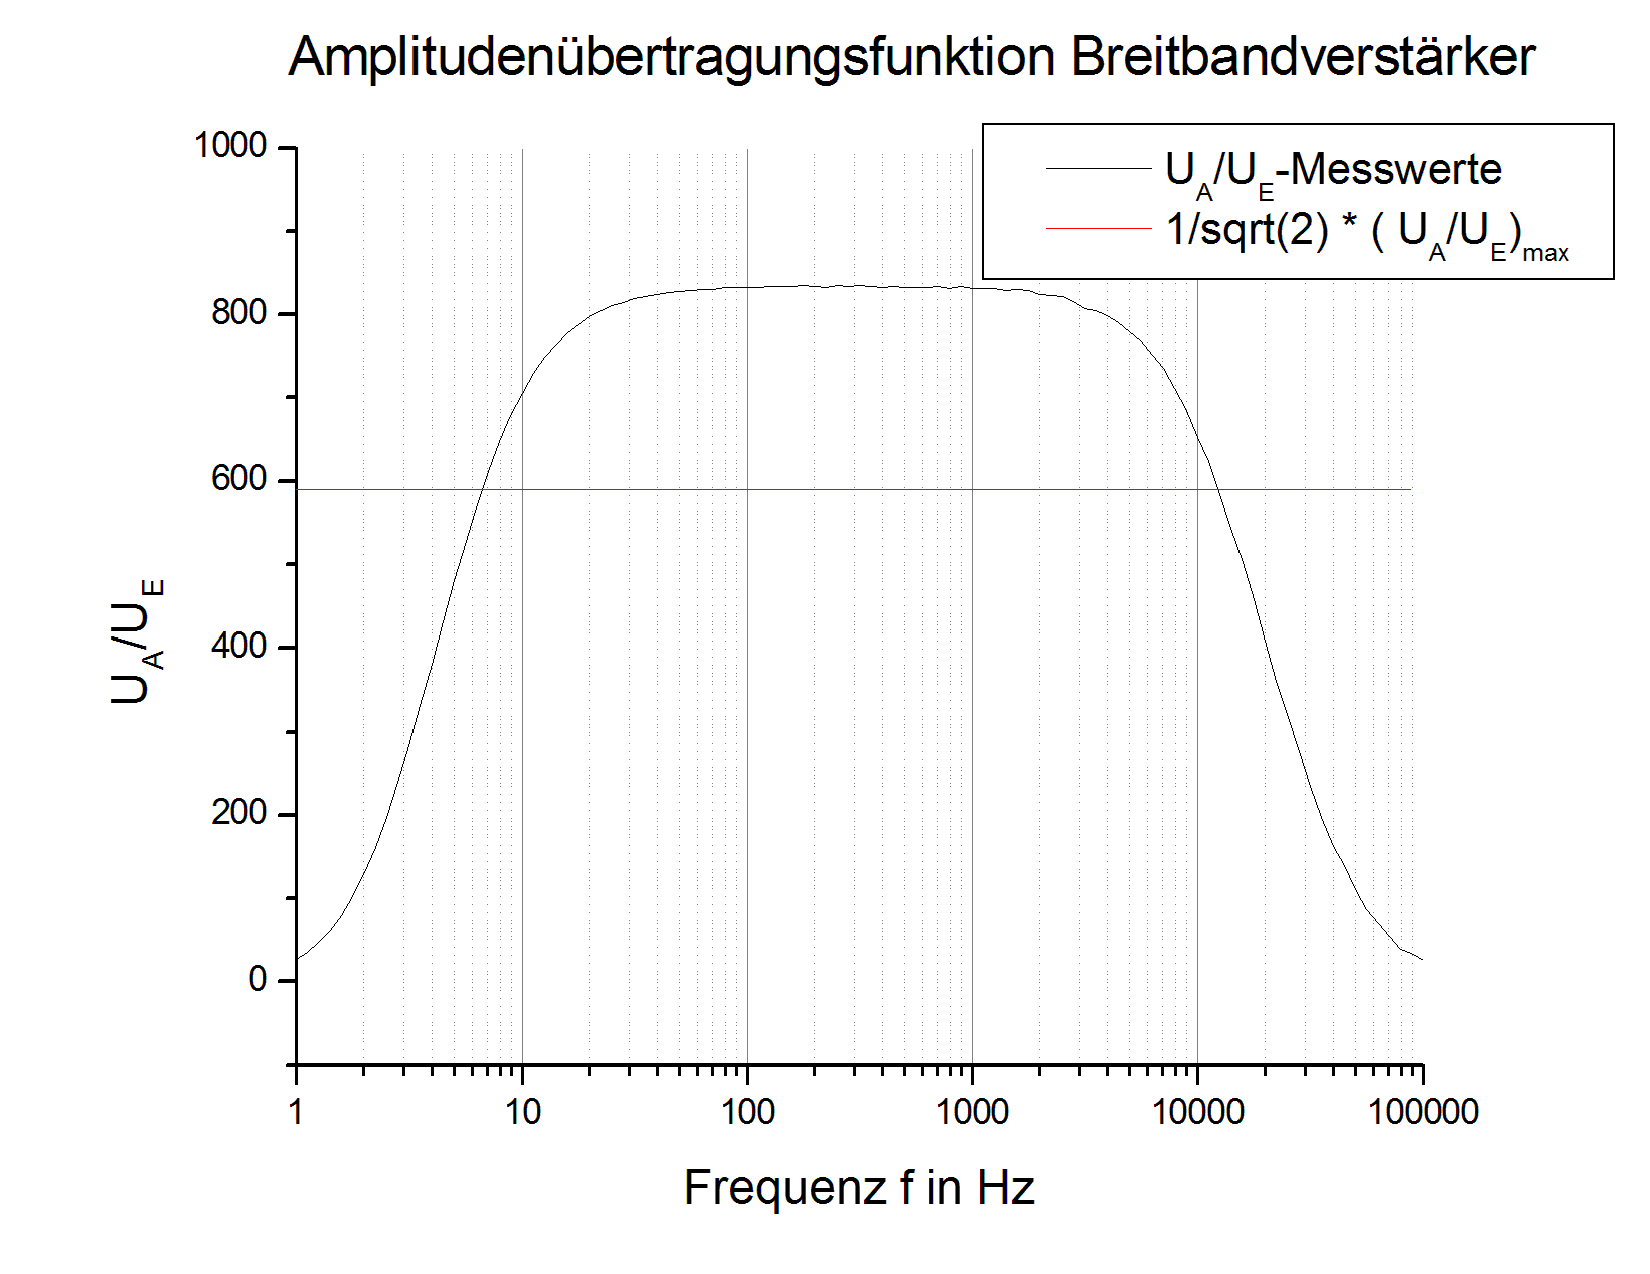
\includegraphics[scale=0.4]{A1a}
				\caption{Amplitudenübertragungsfunktion Breitbandverstärker}
			\end{figure}
			In das Diagramm ist zusätzlich eine Gerade eingezeichnet, welche den $ \frac{U_{max}}{\sqrt{2}} $ anzeigt. Die Schnittpunkte dieser Geraden mit der Amplitudenübertragungsfunktion ergeben die obere und untere Grenzfrequenz $ f_{unten} $ und $ f_{oben} $. Die Differenz beider liefert uns die gesuchte Bandbreite unseres Breitbandverstärkers.
			\begin{equation*}
				\Delta f=f_{oben}-f_{unten}=11500 \ Hz - 7 \ Hz = 11493 \ Hz
			\end{equation*}
			\newline
			Als nächstes sollten die beiden TT-Filter für 25Hz und 180Hz untersucht werden. Auch dazu wurden die Amplitudenübertragungsfunktionen aufgenommen. Daraus lassen sich analog die obere und untere Grenzfrequenz ablesen, sowie die Bandbreite berechnen. Die Güte der Filter ergibt sich nach $ Q=\frac{f_{Grenz}}{\Delta f} $. Der 25Hz-TT-Filter wurde mit einer Spannungsamplitude von $10 \ mV_{pp}$ und der 180Hz-TT-Filter mit $1\ V_{pp}$ gemessen. Es ergaben sich die folgenden Verläufe.
			\clearpage
			\begin{figure}[h!]
					\centering
					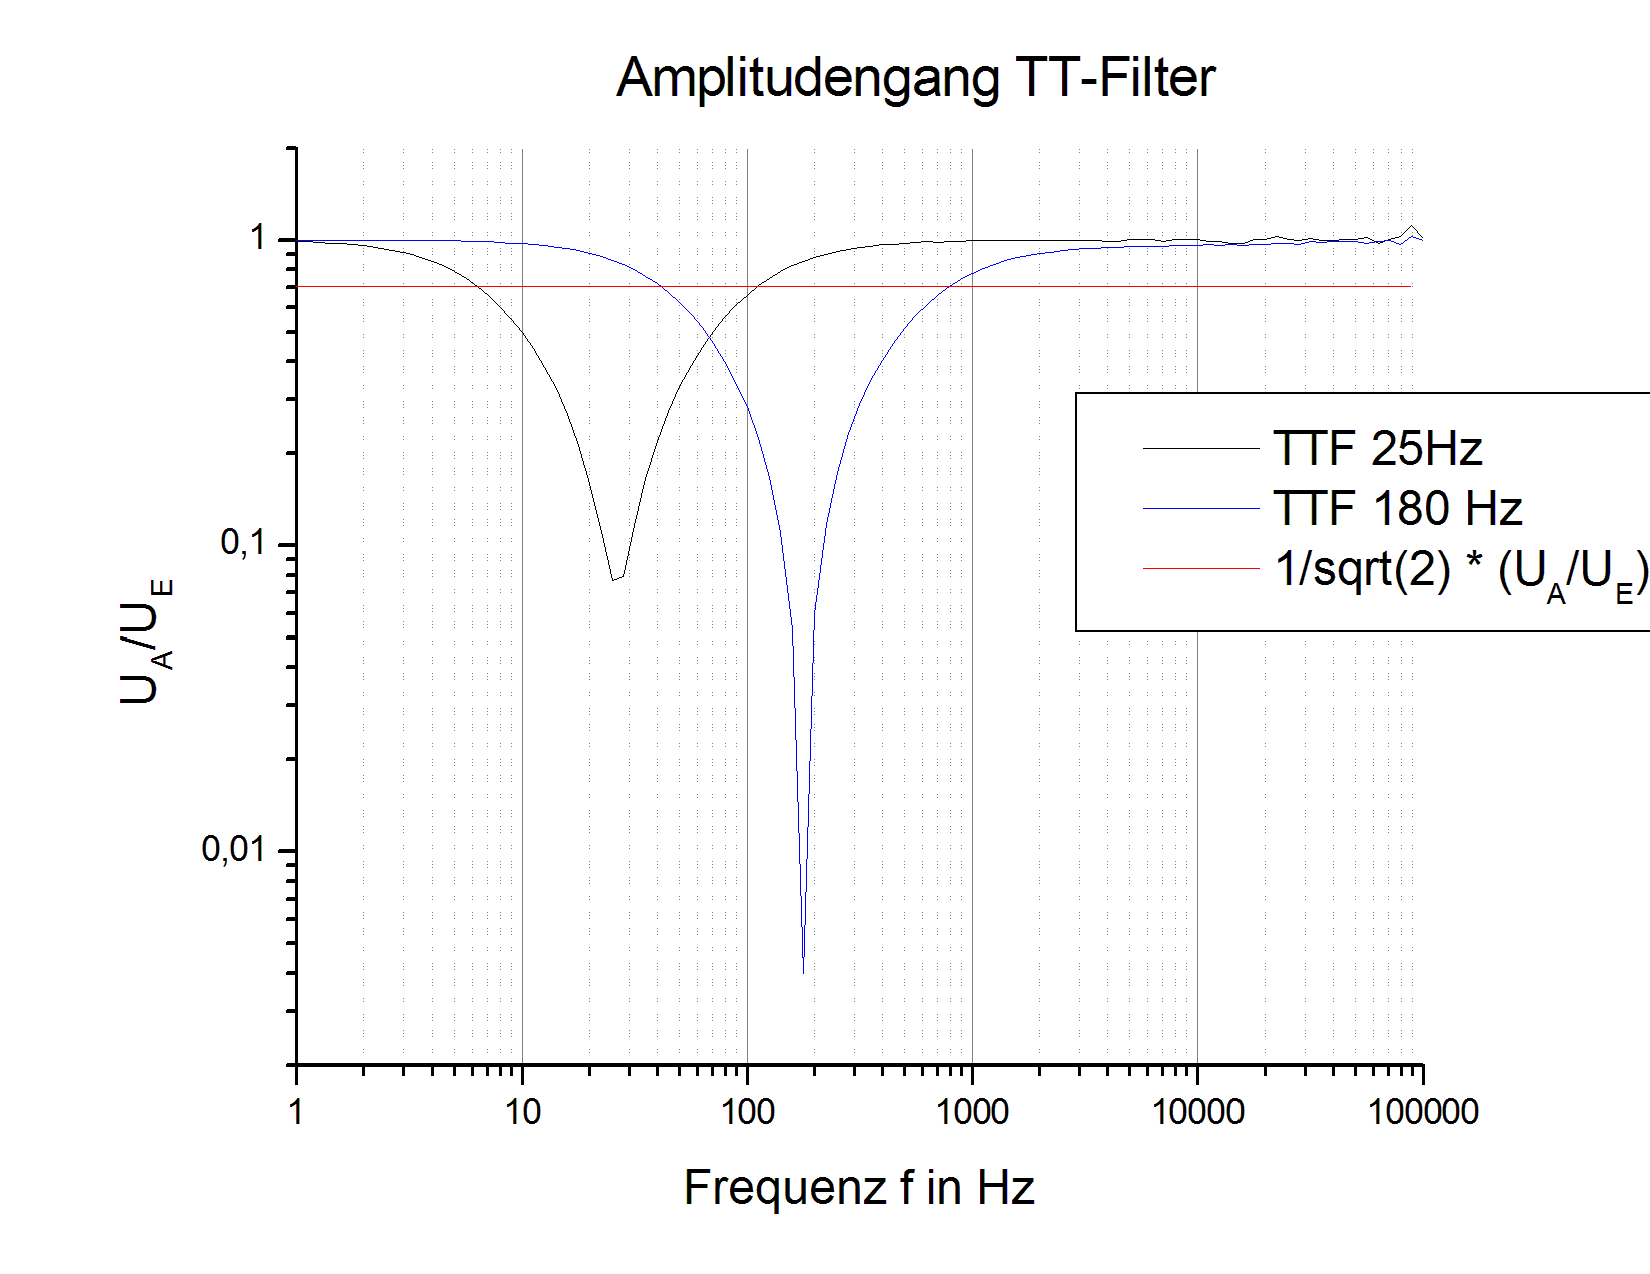
\includegraphics[scale=0.4]{A1b}
					\caption{Amplitudenübertragungsfunktion TT-Filter}
			\end{figure}
			
			In der Tabelle sind alle Werte zusammengefasst:
			\center
			\begin{tabular}{|c|c|c|c|c|}
			\hline $f_{grenz} $ in Hz & $f_{unten}$ in Hz & $f_{oben}$ in Hz & $\Delta f$ in Hz & Güte Q \\ 
			\hline 25 & 6,2 & 110 & 103,8 & 0,241 \\ 
			\hline 180 & 41 & 800 & 759 & 0,237 \\ 
			\hline 
			\end{tabular} 
			\flushleft
			
			Anschließend haben wir  in Aufgabe 1.1.c den TT-Filter für 180Hz in die Rückkopplung des Bandbreitenverstärkers eingefügt. Für den dadurch entstandenen Schmalbandverstärker haben wir für drei Rückkopplungsgrade von 3,5 und 7 (=Stellradeinstellung) den Amplitudengang aufgenommen. Daraus kann man abermals die Grenzfrequenzen, die Bandbreite und die Güte bestimmen. Die Daten sind in der folgenden Tabelle zusammengefasst.
			\center
			\begin{tabular}{|c|c|c|c|c|c|}
			\hline Rückkopplungsgrad & $f_{grenz}$ in Hz & $f_{unten}$ in Hz & $f_{oben}$ in Hz & $\Delta f$ in Hz & Güte Q \\ 
			\hline 3 & 230 & 130 & 426 & 296 & 0,777 \\ 
			\hline 5 & 210 & 130 & 300 & 170 & 1,240 \\ 
			\hline 7 & 200 & 130 & 240 & 110 & 1,818 \\ 
			\hline 
			\end{tabular}
			\flushleft Die Werte liesen sich aus dem nachfolgendem Diagramm ablesen. Die Ablesefehler werden hierbei vernachlässigt.
			\begin{figure}[h!]
					\centering
					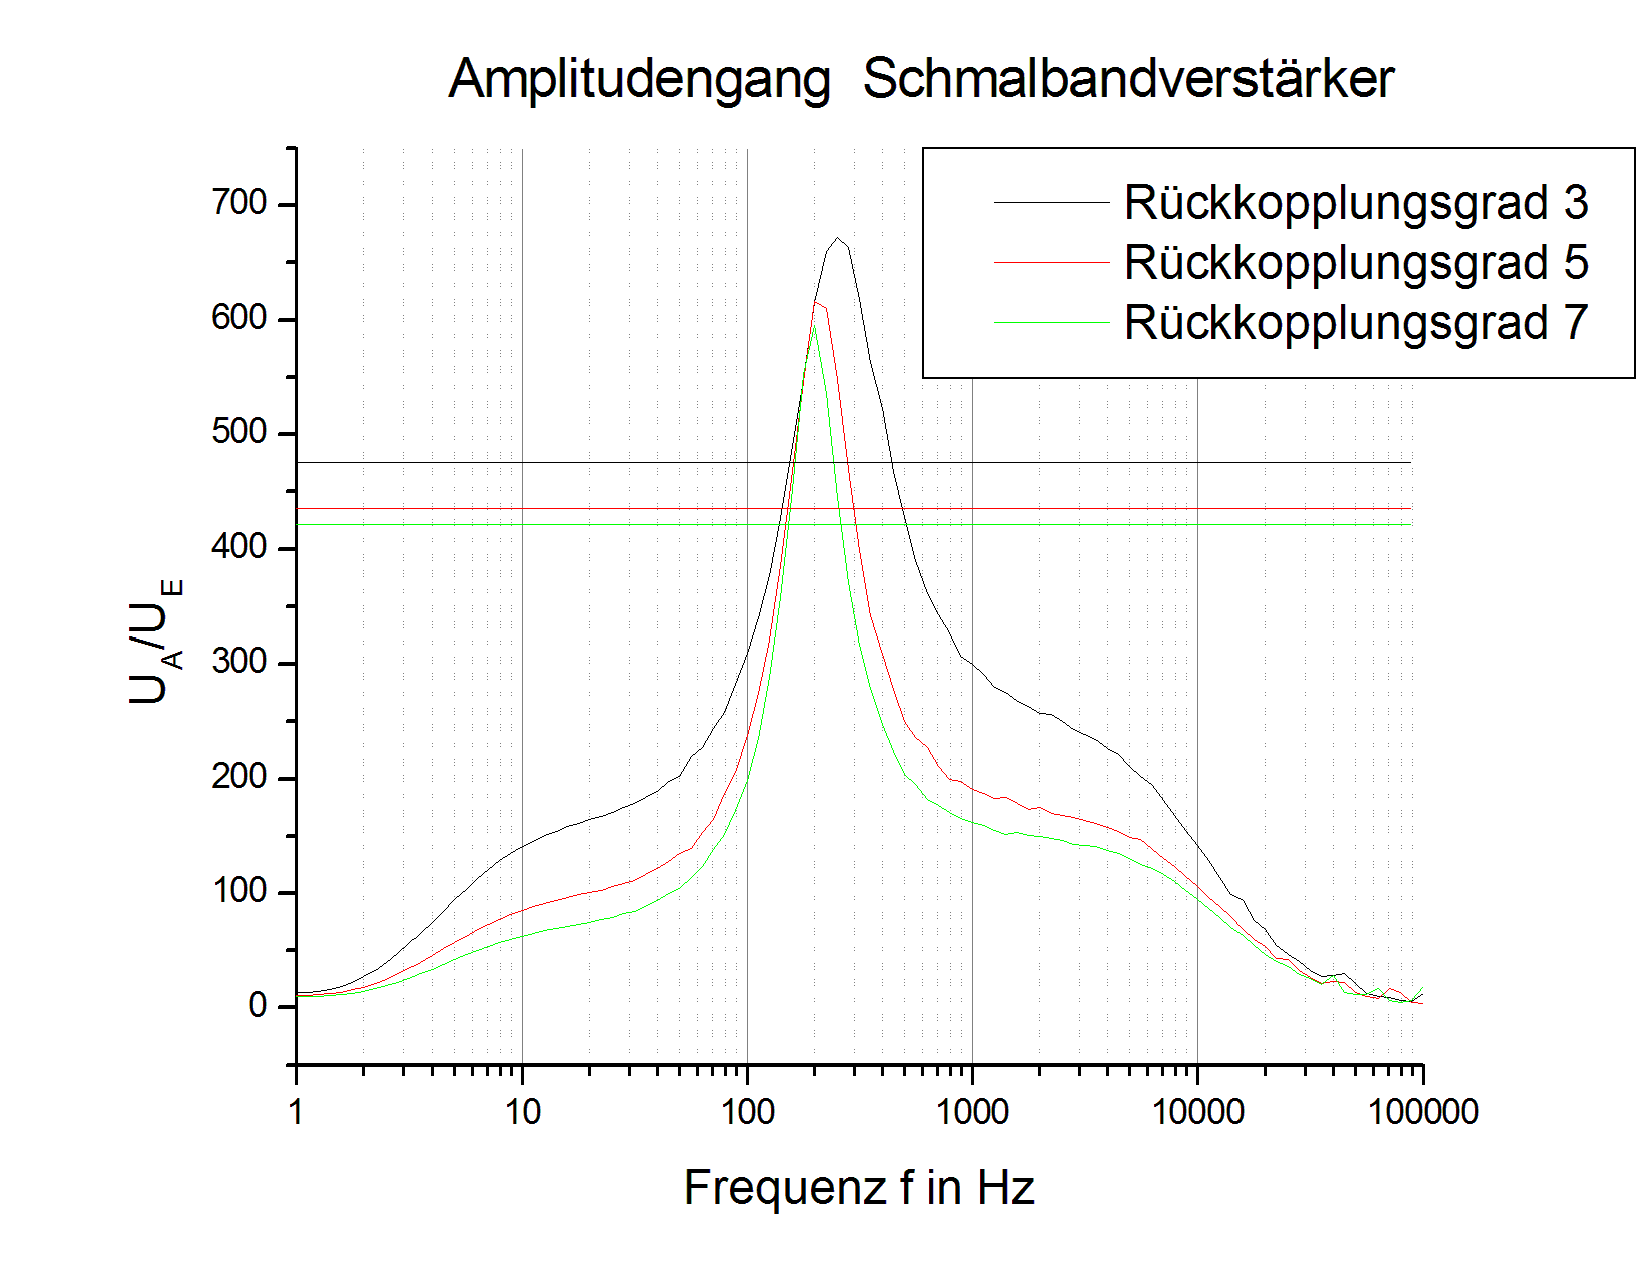
\includegraphics[scale=0.4]{A1c}
					\caption{Amplitudengang Schmalbandverstärker für versch. Rückkopplungsgrade}
			\end{figure}
			
			Mit steigendem Rückkopplungsgrad steigt auch die Güte des Schmalbandverstärkers. Im Vergleich zu dem Breitbandverstärker hat sich die Güte mehr als verdreifacht (von 0,24 auf 0,78 bei dem geringsten vermessenen Rückkopplungsgrad).\\
			
			Um in Aufgabe 1.1.d die maximale Phasenverschiebung zu bestimmen, welche mit dem vorliegenden Phasenschieber bei 180Hz Referenzsignal zu erreichen ist, haben wir das Referenzsignal an das Oszilloskop auf Kanal 1 und den Ausgang des Phasenempfindlichen Gleichrichters (PEG), der mit 5V und 0V gespeist wurde, auf Kanal 2 gelegt. Im DUAL-Modus konnten nun zwischen den beiden Signalen die zeitliche Verschiebung gemessen werden, welche sich gemäß 
			\begin{equation*}
				\frac{\Delta t}{T}=\frac{\Delta \phi}{360^\circ} \ \ \ \ \Rightarrow \ \ \ \ \Delta \phi=f\cdot \Delta t \cdot 360^\circ
			\end{equation*}
			in eine Phasenverschiebung umrechnen lässt. Es wurden folgende Werte gemessen.
			\center
			\begin{tabular}{|c|c|c|c|}
			\hline U in V & Stellrad Phase & $\Delta t$ in ms & $ \Delta \phi$ in $^\circ$ \\ 
			\hline 0 & 8 & 2,96 & 191,8 \\ 
			\hline 0 & 13 & 0,41 & 26,6 \\ 
			\hline 5 & 8 & 0,19 & 12,3 \\ 
			\hline 5 & 13 & 2,45 & 158,8 \\ 
			\hline 
			\end{tabular} 
			\flushleft
			Folglich lässt sich für 0V am PEG und ein Referenzsignal von f=180Hz eine maximale Phasenverschiebung von $ 191,8^\circ $ und für 5V eine von $ 158,8^\circ $ einstellen.\\
			
			In Aufgabe 1.1.e sollte nun die Gleichrichtungswirkung des PEG untersucht werden. Dafür nahmen wir Bilder bei Einwegegleichrichtung und Zweiwegegleichrichtung auf.
			\clearpage
			Zunächst für die Einwegegleichrichtung:
			
			\begin{figure}[h!]
				\centering
				\subfigure[$Einwegegleichrichtung: \Delta \phi = 0^\circ $]{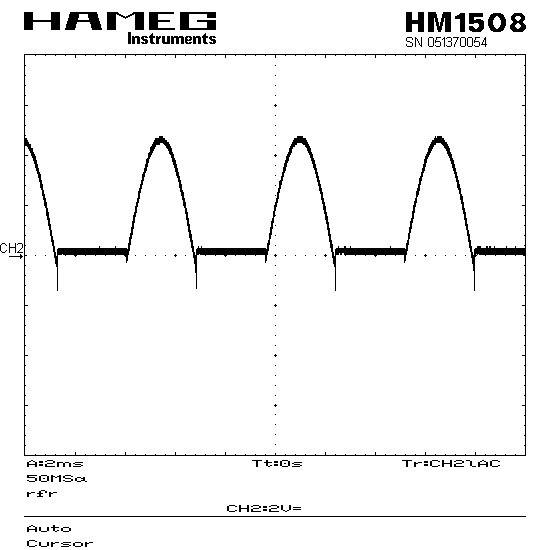
\includegraphics[scale=0.4]{SCR00018}}
				\subfigure[$ \Delta \phi = -90 ^\circ $]{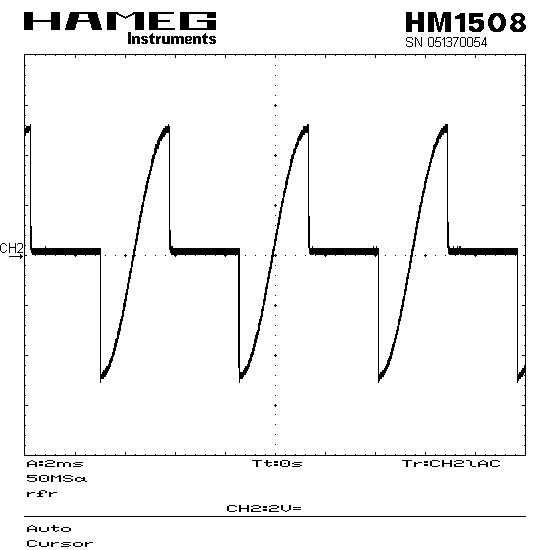
\includegraphics[scale=0.4]{SCR00019}}
			\end{figure}
			
			Im Prinzip kann man sich die Einwegegleichrichtung vorstellen wie eine Überlagerung/Multiplikation von einem Sinus mit einem Rechtecksignal, welches immer zwischen 0 (AUS) und 1 (AN) hin und her springt. Im linken Bild ist die Phasenverschiebung zwischen Sinus und Rechteck genau $ \Delta \phi = 0^\circ $ und im rechten Bild $ \Delta \phi =-90^\circ \simeq 270^\circ$.\\
			Die Zweiwegegleichrichtung ergibt die folgenden Bilder für $ \Delta \phi = 0^\circ $ und $ \Delta \phi = 270^\circ $:
			
			\begin{figure}[h!]
				\centering
				\subfigure[$Zweiwegegleichrichtung: \Delta \phi = 0^\circ $]{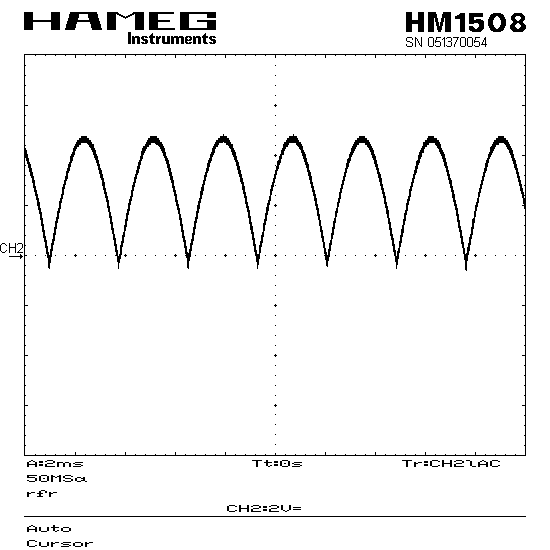
\includegraphics[scale=0.4]{SCR00020}}
				\subfigure[$ \Delta \phi = -90 ^\circ $]{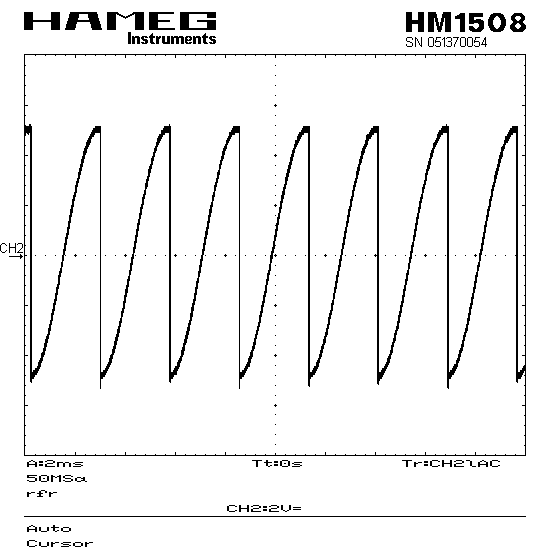
\includegraphics[scale=0.4]{SCR00021}}
			\end{figure}
			
			Anschießend untersuchten wir die Funktion des nachgeschalteten Tiefpasses. Diese wurde anhand der folgenden Bilder deutlich. Für die obigen Phasenverschiebungen und einen Tiefpass aus einem Widerstand mit $ R=18\ k\Omega $ und einem Kondensator mit $ C=10 \ \mu F $, haben wir Bilder aufgenommen. Nach Durchlauf durch den Kondensator ergaben sich für Zweiwegegleichrichtung folgende Verläufe.
			 \begin{figure}[h!]
			 \centering
			 	\subfigure[Signal nach Tiefpass:$\Delta \phi = 0^\circ $]{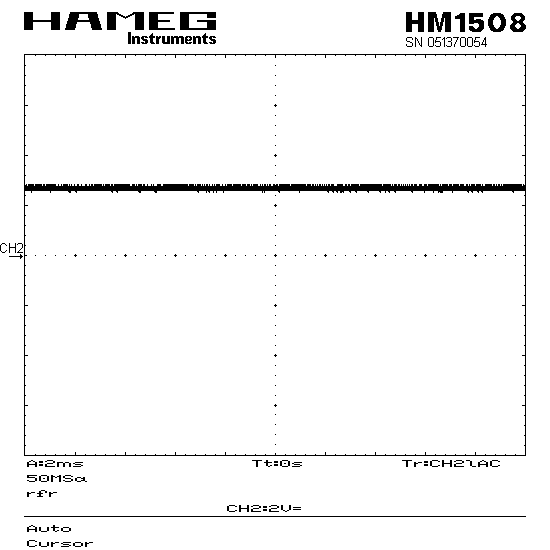
\includegraphics[scale=0.4]{SCR00022}}
			 	\subfigure[$ \Delta \phi = -90 ^\circ$]{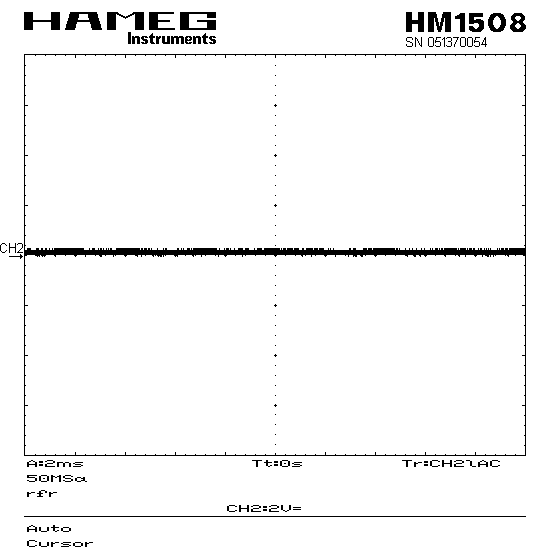
\includegraphics[scale=0.4]{SCR00023}}
			 \end{figure}
			 \newline
			 Ein Tiefpass mit hinreichend großer Zeitkonstante, hier $ \tau =RC=0,18 \ \Omega \cdot F $ erzeugt eine Gleichspannung, welche für $ \Delta \phi =0^\circ $ maximal, für $ \Delta \phi = \pm 90^\circ $ Null und für $ \Delta \phi =180^\circ $ minimal ist. Im Frequenzbereich wird Rauschen höherer Frequenzen durch den Tiefpass unterdrückt, sodass nach der Gleichrichtung nur noch das schmale Frequenzband um f=0 vorliegt.
			 \newline \\
			 In Versuchsteil 1.1.g sollte nun noch der Nachverstärker charakterisiert werden. Dazu nahmen wir eine Amplitudenübertragungsfunktion auf, woraus sich die Bandbreite bestimmen lässt. Da wir nur den rechten Zweig aufgenommen haben, lässt sich nur die obere Grenzfrequenz ablesen als $ f_{oben}=280\ kHz $. Als Bandbreite verwende ich nun einfach 2 mal die obere Grenzfrequenz, als ob der Graph symmetrisch zu f=0 Hz wäre. Diese Annahme ergibt eine Bandbreite von $ \Delta f =560\ Hz $.
			 \begin{figure}[h!]
				 \centering
				 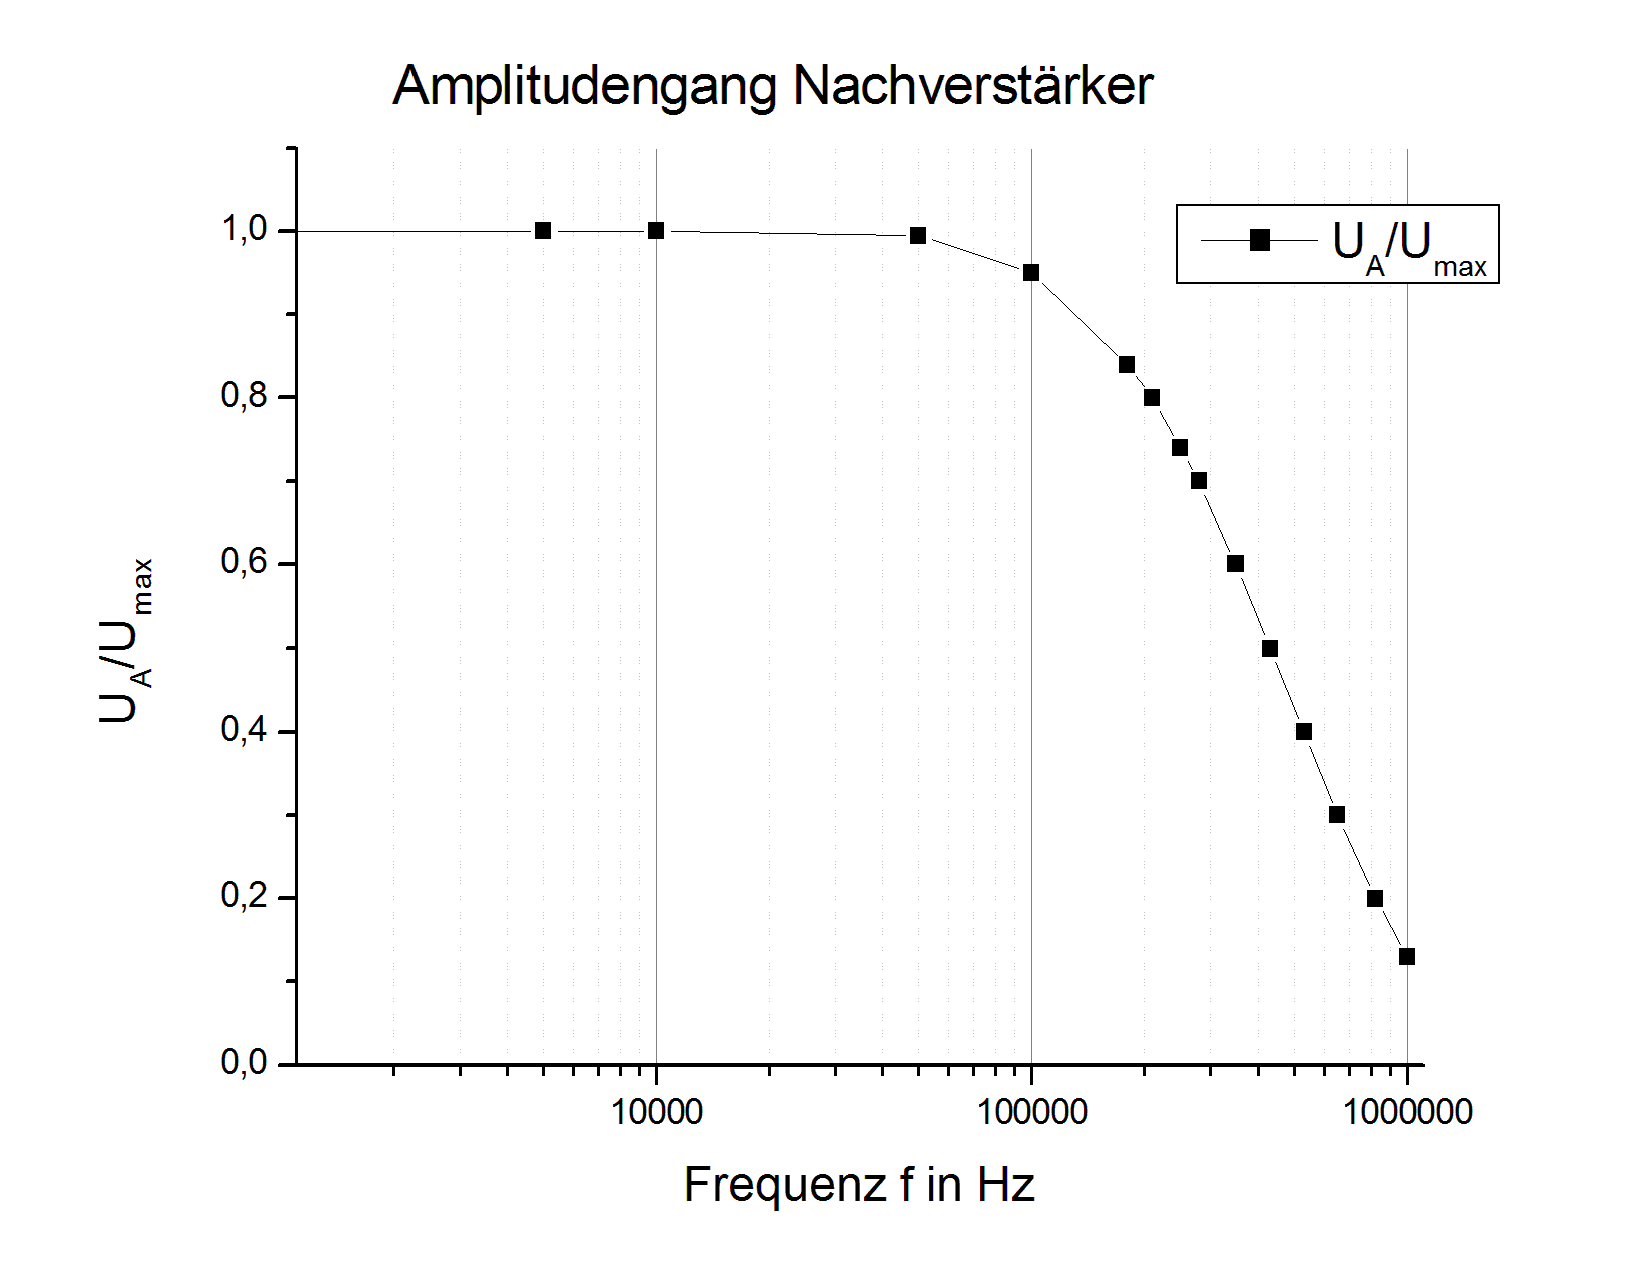
\includegraphics[scale=0.3]{A1g}
				 \caption{Amplitudengang Nachverstärker}
			 \end{figure}
			 
			 In Aufgabe 1.2.1 sollte nun experimentell die Bandbreite des Lock-in bestimmt werden.
			 Dazu haben wir keine ganze Amplitudenübertragungsfunktion aufgezeichnet, sondern nur die Grenzfrequenz $ f_{g} $ und die Werte für $ U=U(f_{g})/\sqrt{2}$, also $ f_{oben} $ und $ f_{unten} $. Dazu verwendeten wir ein Referenzsignal von f=180Hz, welches vom Hameg-Generator erzeugt wurde. Als Signal-Generator diente der Agilent-Generator.
			 Für einen Tiefpass-Widerstand von $ R=560 \ k\Omega $ bestimmten wir: \\
			 $ f_{g}=180,053 \ Hz$,$f_{unten}=180,038 \ Hz $ und $f_{oben}=180,150 \ Hz$ .
			 Daraus lässt sich eine Bandbreite von $ \Delta f = 0,112 \ Hz$ bestimmen.\\
			 Für $ R=2,4 \ M\Omega$ war eine Messwertaufnahme nicht möglich, da der Hameg nicht konstant war und uns das Signal immer weggedriftet ist.
			 \newline
			 Die Aufgabe 1.2.2 haben wir aus zeitlichen Gründen nicht mehr bearbeiten können. Zu erwarten gewesen wäre, dass der Lock-in bis zu einem Signal-Rausch Verhältnis von etwa $ 10^{-6} $ Signale nachweisen kann.
			
		\subsection{Versuchstag 2 - Anwendung des Lock-in-Verstärkers}
			
			\subsubsection{Aufgabe 1.1 - Lock-in als Spektralanalysator}
			Zunächst sollte in Aufgabe 1.1.a ein durch den Agilent erzeugtes Rauschsignal an den Eingang des Lock-in gelegt werden, und für zwei Messfrequenzen die spektrale Rauschamplitude des Eingangssignals bestimmt werden. In Aufgabe 1.1.b soll anschließend noch die Verstärkung des Lock-in kalibriert werden. Dazu erzeugten wir mit dem Hameg ein Referenzsignal von f=180Hz, welches zu Beginn eine Amplitude von $ U_{Hameg}=U_{Referenz}=4,21 \ V_{pp} $ besaß. Die Amplitude des Rauschens war $ U_{Rauschen}=U_{Agilent}=300 \ mV_{pp} $. Da die Spannung des Hameg zu groß war, regelten wir diese über einen Spannungsteiler herunter. Die resultierende Spannung berechnet sich nach 
			\begin{equation*}
					U_{neu}=\frac{11\Omega \cdot U_{Hameg}}{R+11\Omega} \approx \frac{U_{Hameg}}{10000} =4,2\cdot 10^{-4} \ V_{pp} 
			\end{equation*}
			an bei einem Widerstand von $ R=100 \ k\Omega$ .
			Mittels eines Mischers konnten wir entweder Rauschen alleine, Rauschen und Referenzsignal oder nur das Referenzsignal betrachten. Allerdings sorgte dieser nochmal wegen eines Spannungsteilers zu einem Abfall der Spannung um den Faktor 10 (aus $ \frac{910 \Omega}{(8.2 \ k\Omega +910\Omega)} \approx 0.1$). Daher kamen am Lock-In-Verstärkers folgende Signale an:
			\begin{itemize}
			\item Eingang: Rauschsignal mit $ U_{Eingang}=\frac{U_{Rauschen}}{10}=\frac{U_{Agilent}}{10}=30 \ mV_{pp}$
			\item Referenzeingang: Sinus mit $ U_{Referenzeingang}\approx \frac{U_{Hameg}}{10 \cdot 10000 }= 0,042 \ mV_{pp}$
			\end{itemize} 
			Das Signal ist deutlich geringer als das Rauschen ($ SNR=\frac{U_{Signal}^2}{U_{Rauschen}^2}=1,96\cdot 10^{-6} $).\newline
			Wir haben die folgenden Diagramme aufgenommen:
			\begin{itemize}
			\item Rauschen: a und b - ohne TT-Filter 180Hz
			\begin{figure}[h!]
			\subfigure[Rauschen Zeitbereich]{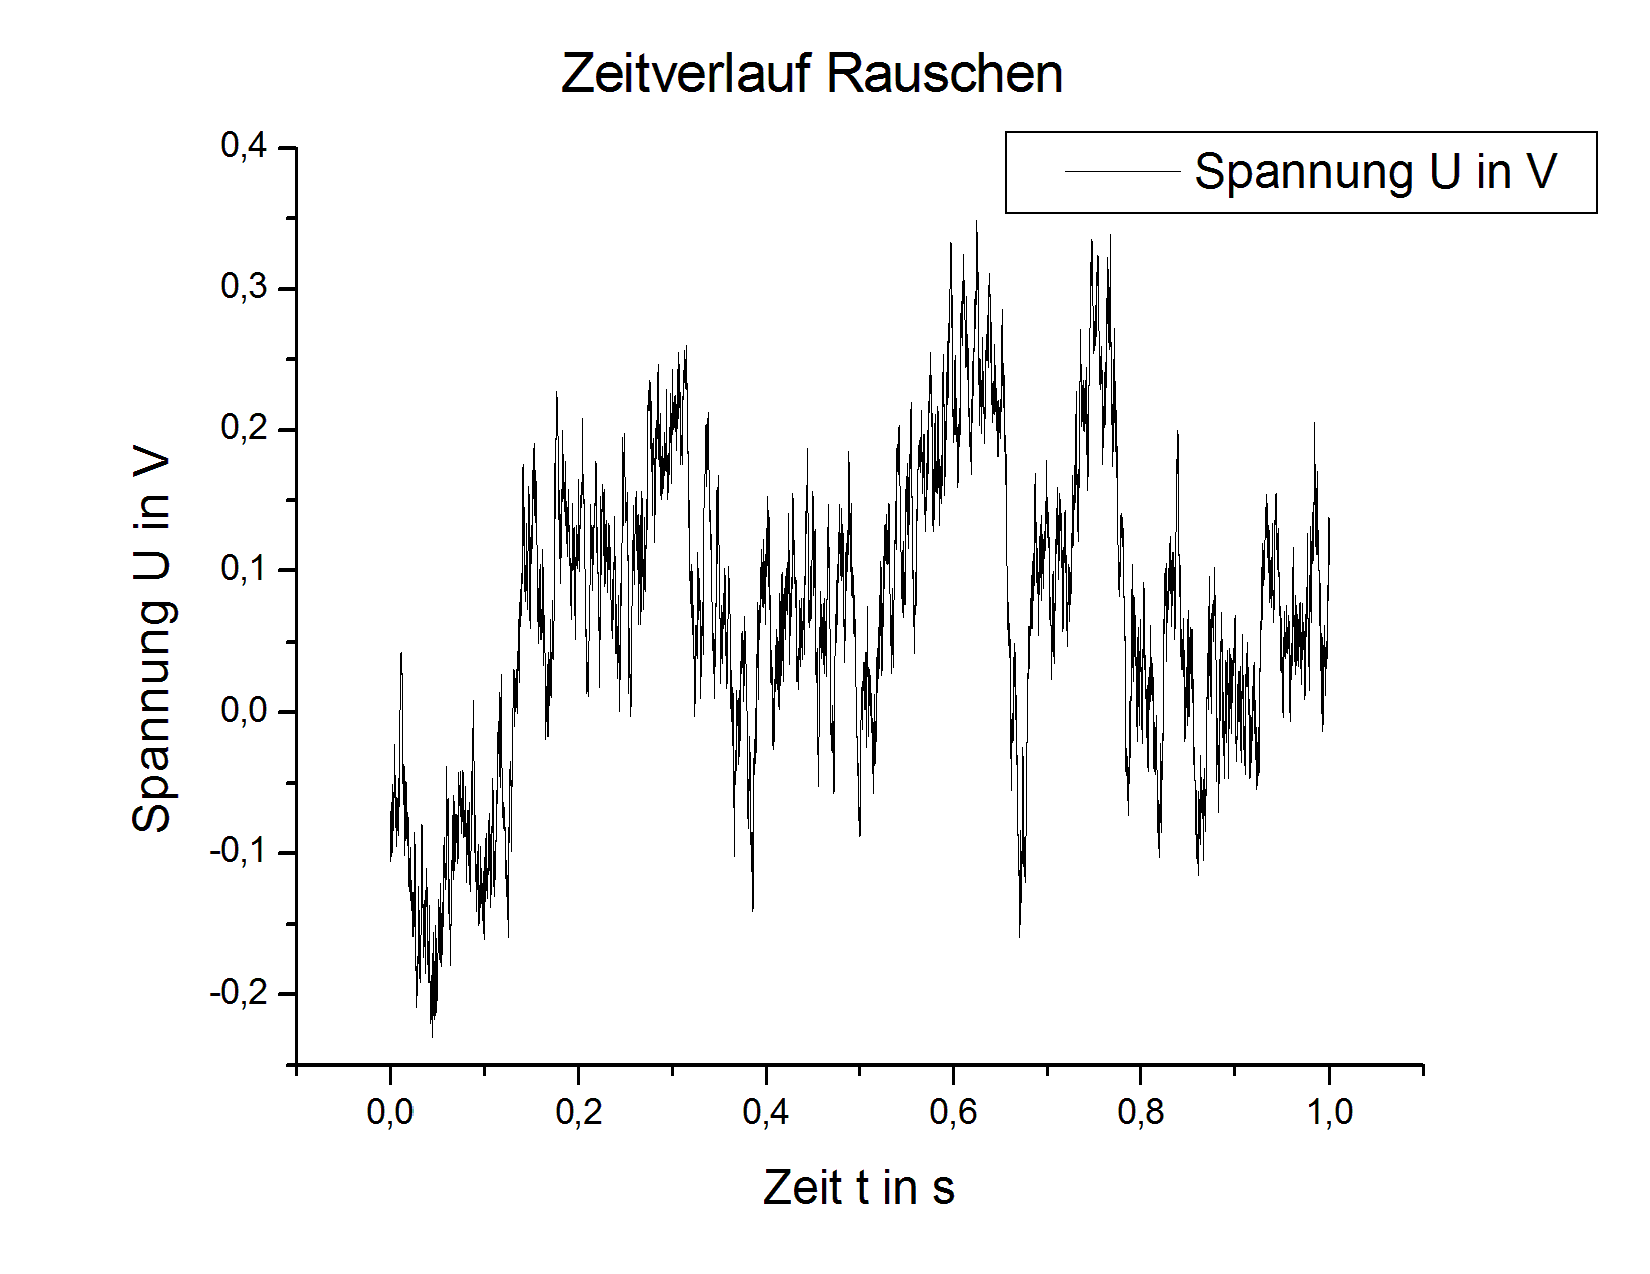
\includegraphics[scale=0.25]{A1aGraph1}}
			\subfigure[Rauschen Frequenzbereich]{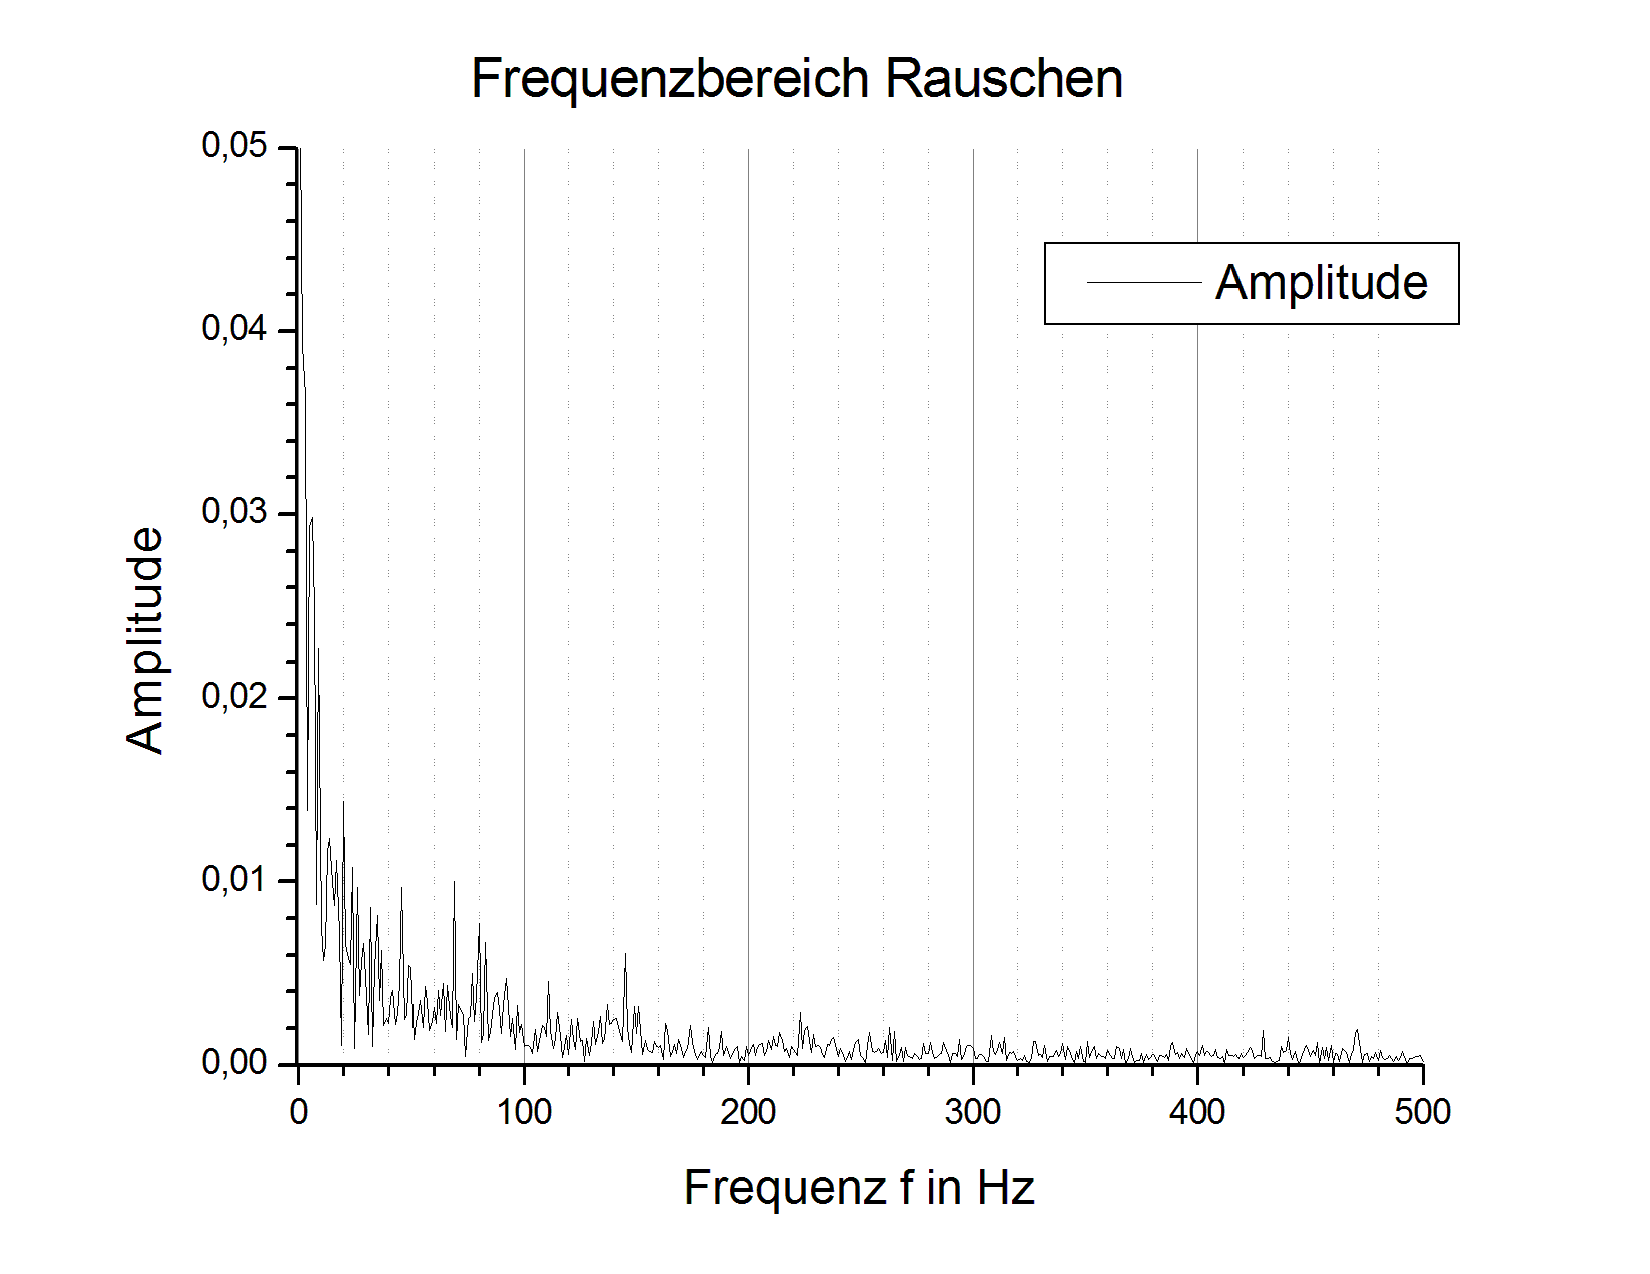
\includegraphics[scale=0.25]{A1a-Graph2}}
			\end{figure}
			\item Rauschen+Referenzsignal: c und d - ohne TT-Filter 180Hz
				\begin{figure}[h!]
						\subfigure[Gemisch Zeitbereich]{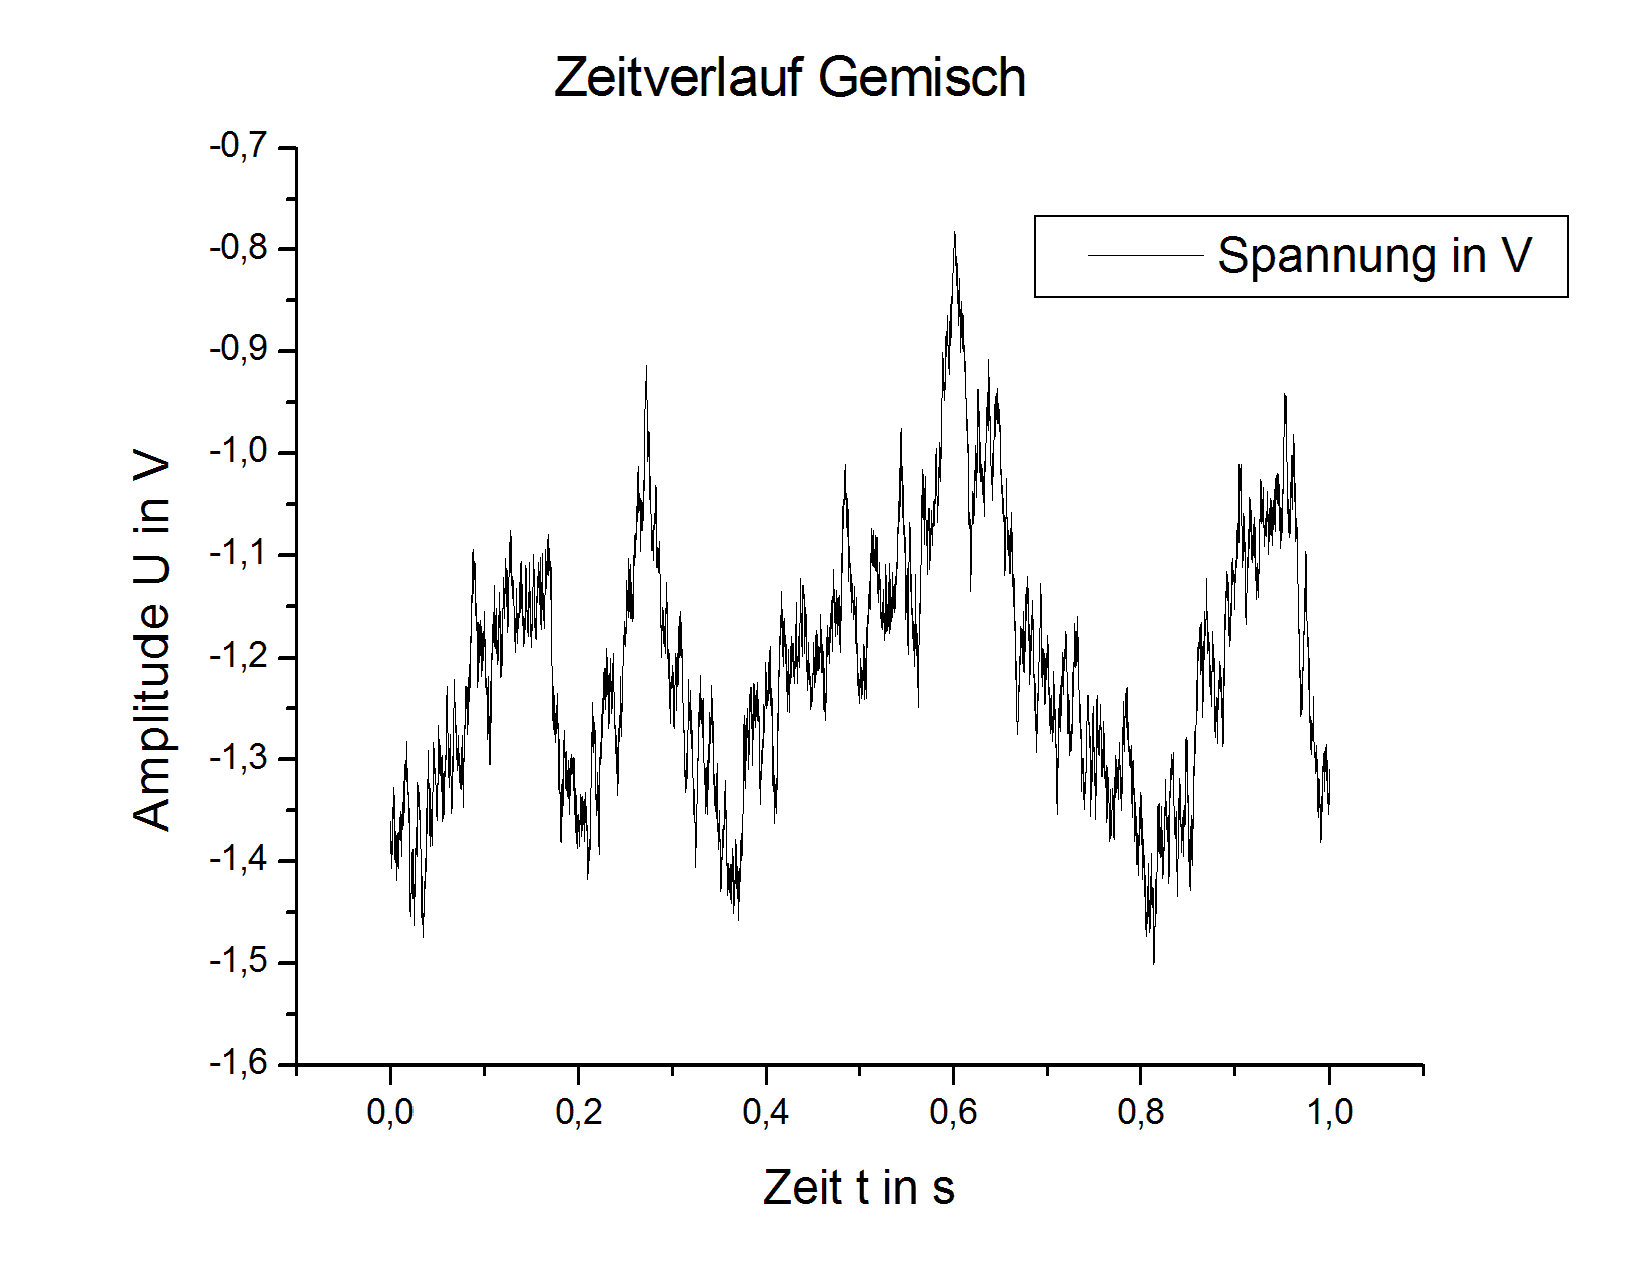
\includegraphics[scale=0.25]{A1aGemischGraph1}}
						\subfigure[Gemisch Frequenzbereich]{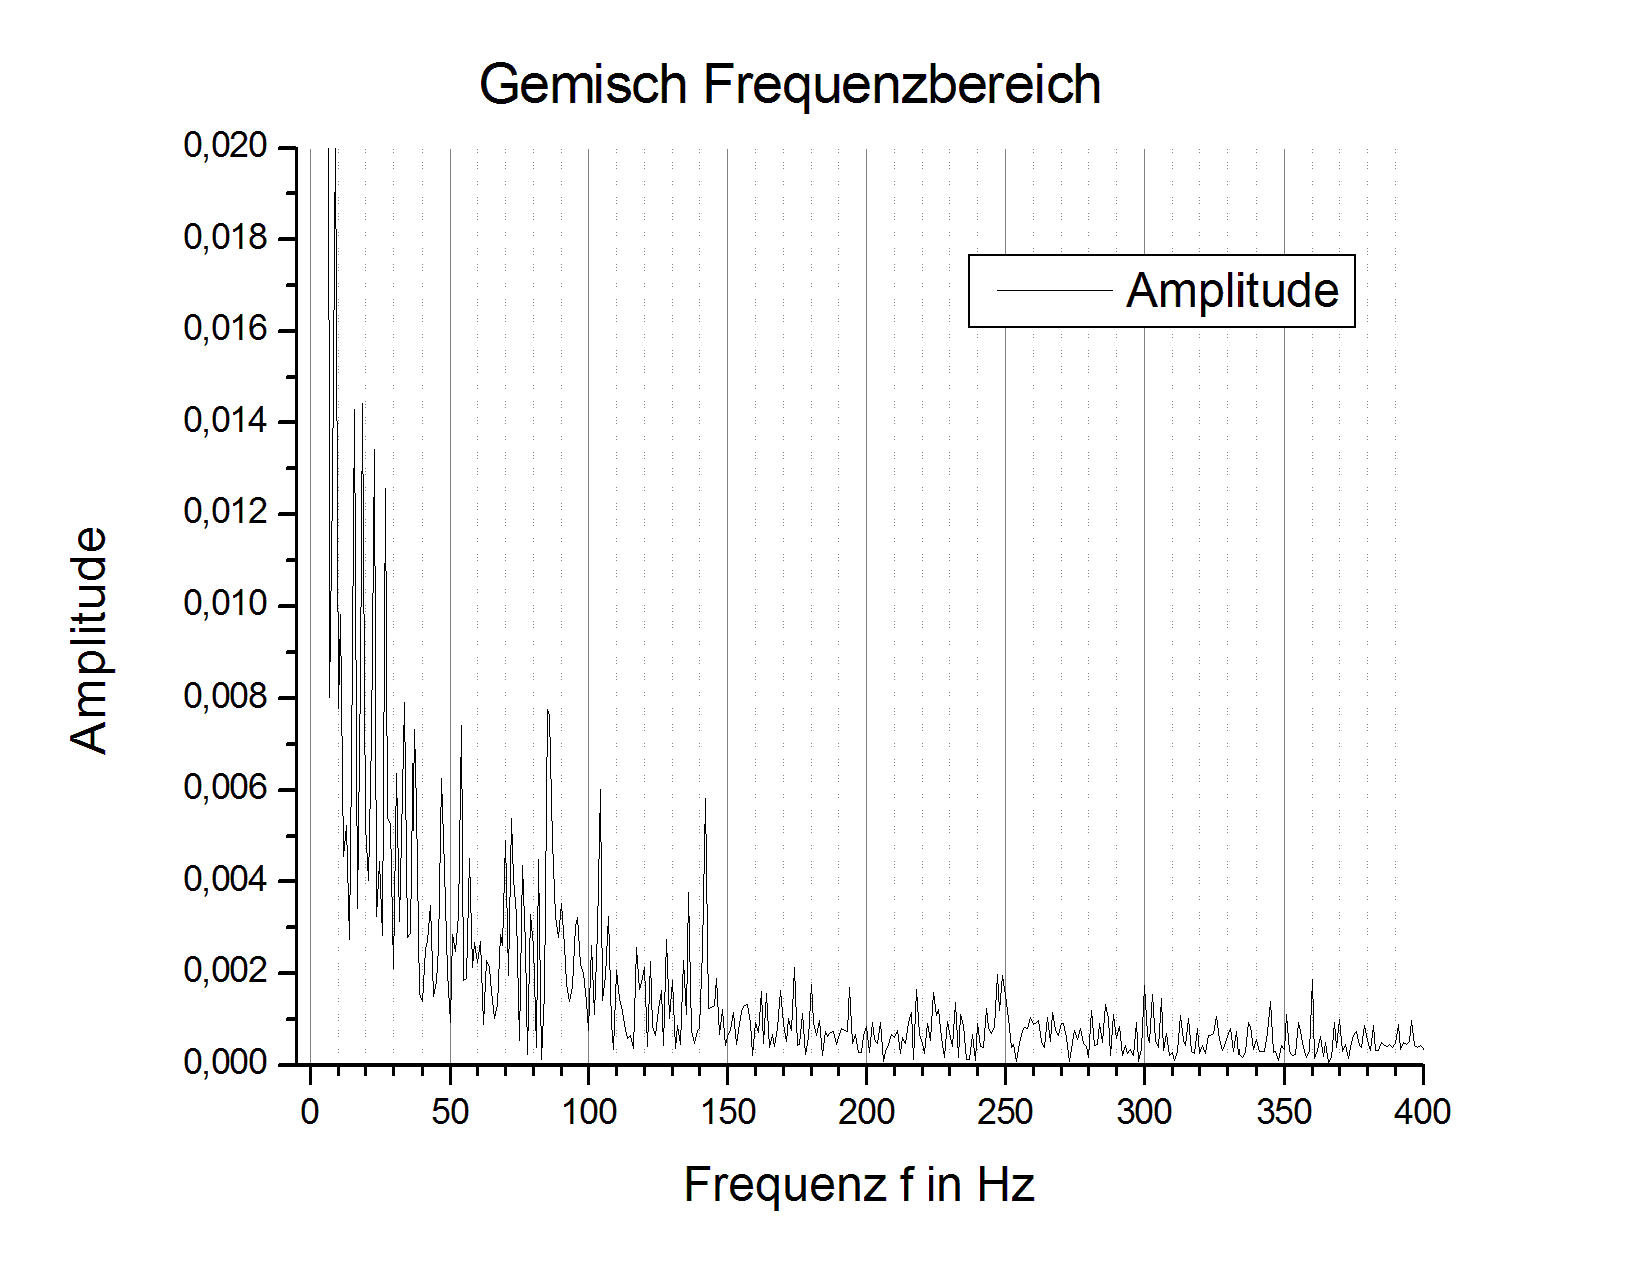
\includegraphics[scale=0.25]{A1aGemisch-Graph2}}
				\end{figure}
			\item Rauschen + Referenzsignal mit TT-Filter 180Hz:
				\begin{figure}[h!]
						\subfigure[Gemisch mit TTF180 Zeitbereich]{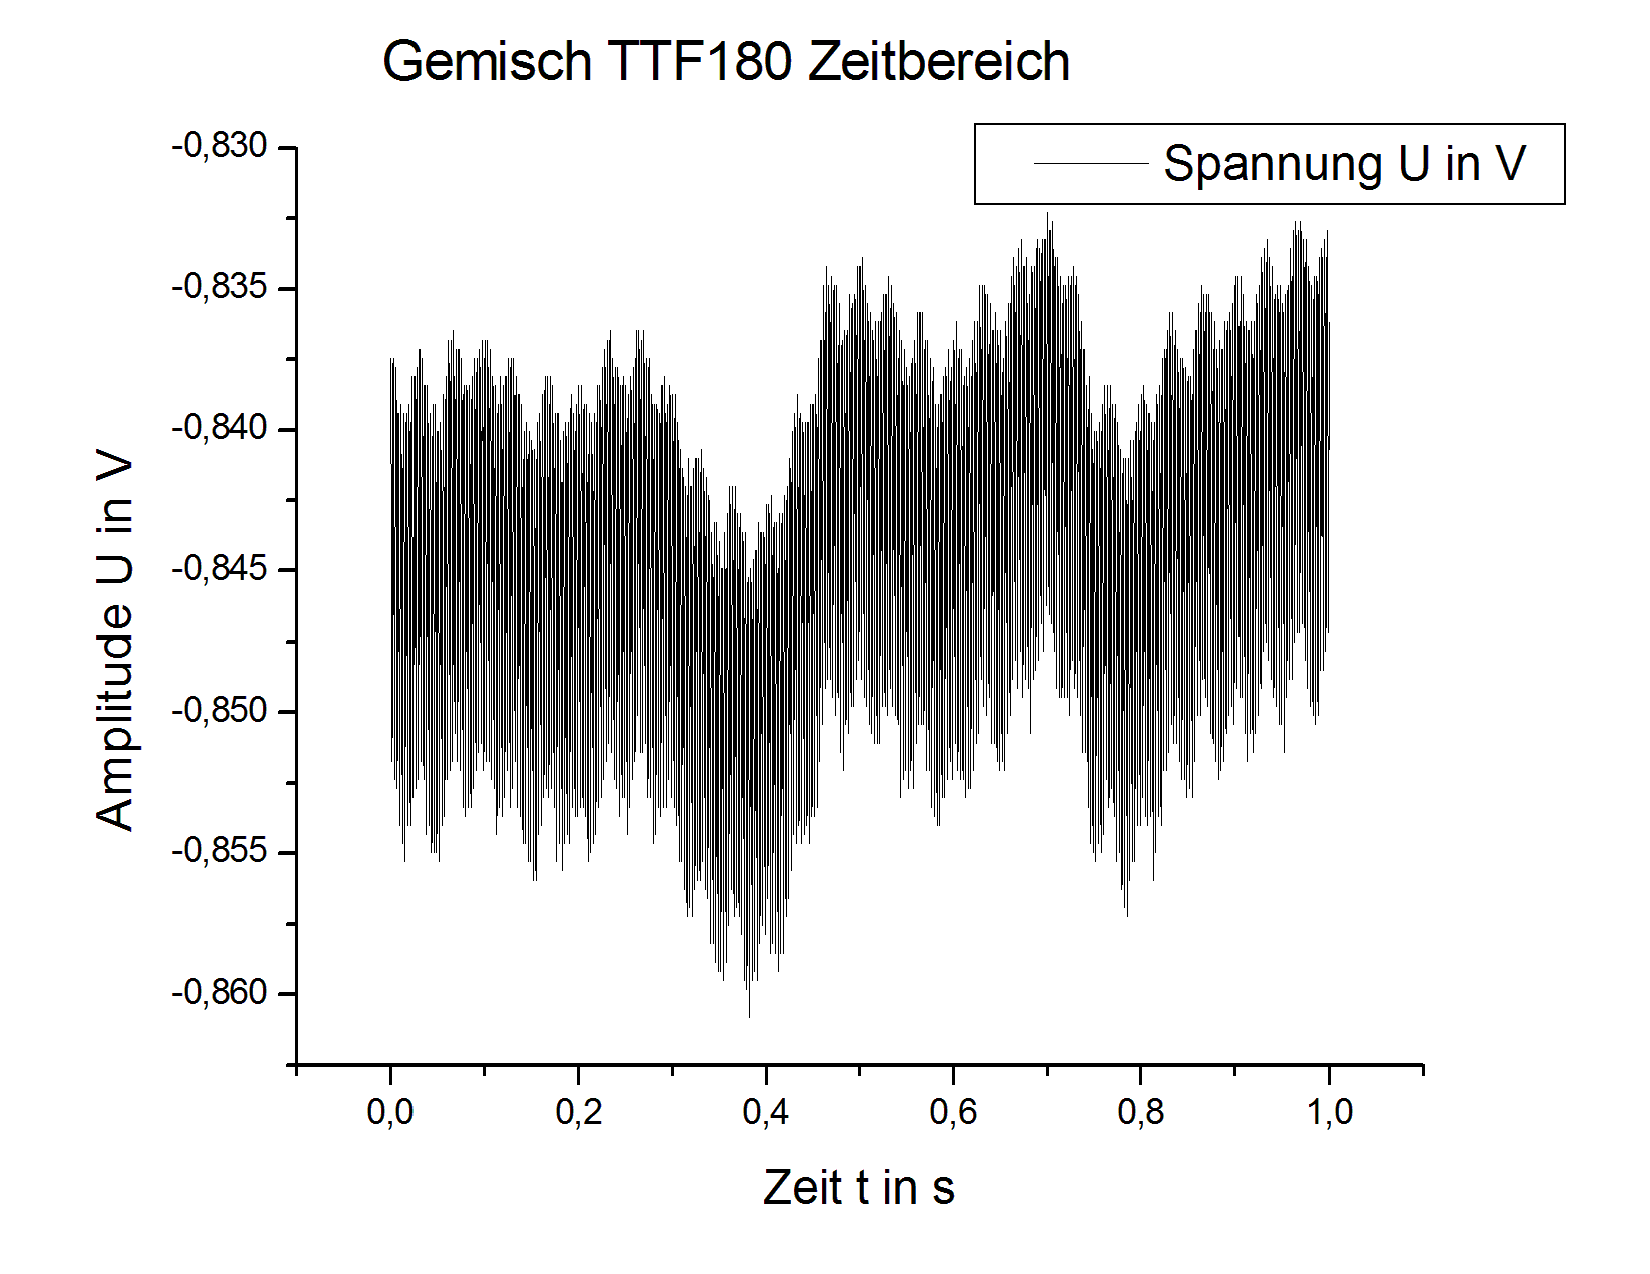
\includegraphics[scale=0.25]{A1aTTF180Graph1}}
						\subfigure[ Gemisch TTF180 Frequenzbereich]{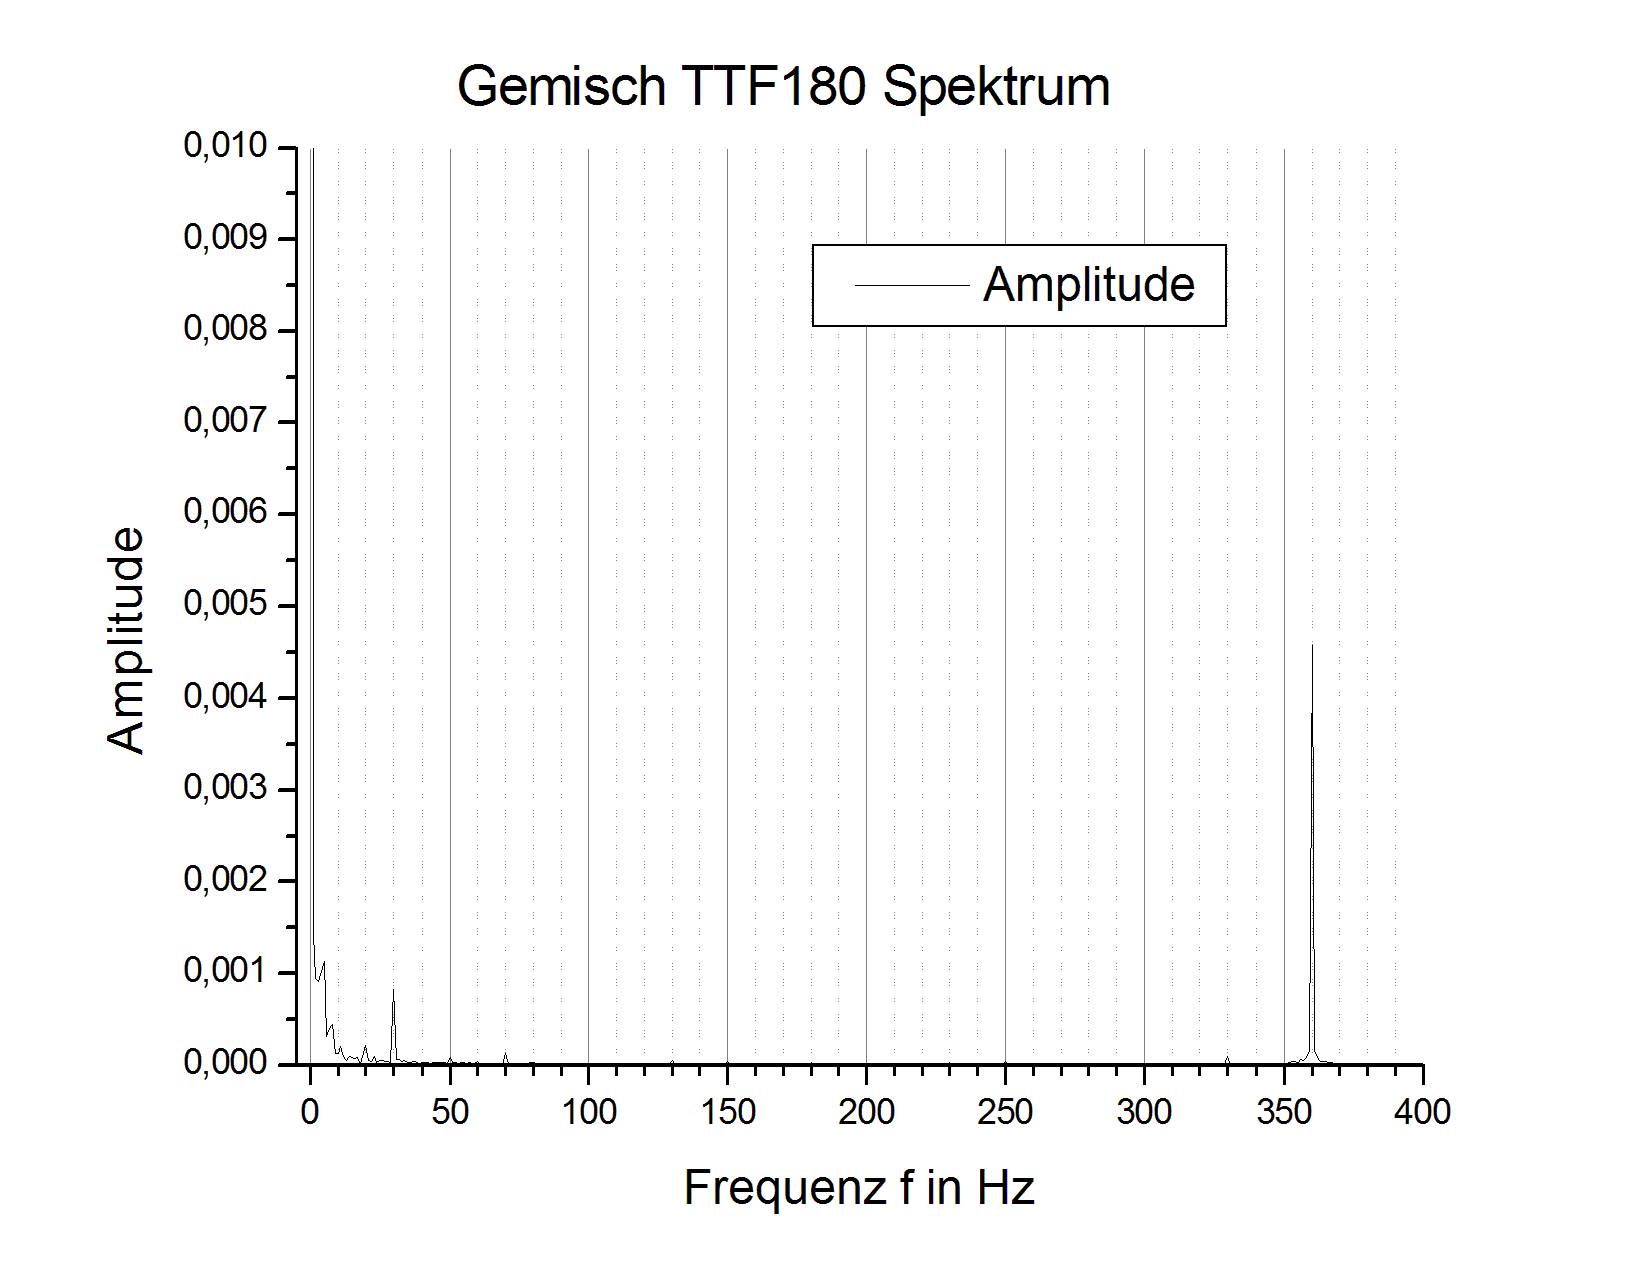
\includegraphics[scale=0.25]{A1aTTF180Gemisch}}
				\end{figure}
			\end{itemize}
			\clearpage
			Für alle Daten wurde ein Tiefpass mit einem Widerstand von $ R=18\,k\Omega $ und einem Kondensator mit $ C=10\, \mu F $ verwendet.
			Aus den Messwerten des Zeitbereichs kann man den Mittelwert, die Standardabweichung und die Varianz berechnen.  Für alle drei Diagramme sind diese hier in nachfolgender Tabelle zusammengefasst.
			\center 
			\begin{tabular}{|c|c|c|c|}
			\hline  & Mittelwert in V & Standardabweichung in V & Varianz in $V^{2}$ \\ 
			\hline Rauschen & 0,0707 & 0,10782 & 0,01162 \\ 
			\hline Rauschen+Referenzsignal & -1,20722 & 0,23692 & 0,01611 \\ 
			\hline Gemisch mit TTF180Hz & -0,84358 & 0,00545 & 2,97E-05 \\ 
			\hline 
			\end{tabular} 
			\flushleft
			Das Rauschen alleine wird durch den Lock-in ohne den TT-Filter um den Faktor 
			\begin{equation*}
			 V=\frac{U_{Ausgang}}{U_{Eingang}}= \frac{0,10782 V }{0,5\cdot 30\cdot 10^{-3}V}=7,2
			\end{equation*} verstärkt [Faktor 0,5 für Umrechnung $ V_{pp} $ zu V].
			Das Gemisch ohne den TT-Filter liefert weder im Frequenzbereich, noch im Zeitbereich einen Hinweis auf das Referenzsignal von f=180Hz. Bei beiden Frequenzbereichen ist jedoch immer ein sehr großer Gleichspannungsanteil bei f=0Hz zu erkennen. Dieser kommt durch das Wirken des PEG (Phasenempfindlichen Gleichrichters).\\
			Erst im Frequenzbereich des Gemischs mit dem TT-Filter für 180Hz lässt sich deutlich ein Peak bei 360Hz, also der doppelten Referenzsignalfrequenz erkennen. Das der Peak bei der doppelten Frequenz liegt, lässt sich durch nachfolgende Rechnung einfach nachvollziehen:
			\begin{align*}
				Additionstheorem: \ \ \ \ \sin (x) \cdot \sin(y)&=\frac{1}{2}\left[\cos (x-y)-cos(x+y) \right] \\
				Fall \ x=y: \ \ \ \ \ \ \ \ \ \ \ \ \sin^2(x)&=\frac{1}{2}\left[1-cos(2x) \right]
			\end{align*}
			Es ergibt sich bei der Überlagerung zweier Signale (hier vereinfacht zwei Sinus und nicht ein Sinus mit Rauschen) - und nichts anderes geschieht im Multiplikator - ein Gleichspannungsanteil $ 0,5 $ und ein Peak bei der doppelten Signalfrequenz $ 0,5\cdot \cos(2x)$.
			Wenn man das weiß, so kann man das Signal von f=180Hz, welches ja deutlich kleiner ist, als das Rauschen [$ \Longrightarrow $ SNR] deutlich identifizieren.
			\newline
			In Aufgabe 1.1.c sollte nun das Spektrum des Rauschens aufgenommen werden.  Dieses ist ein einfaches weißes Rauschen mit den charakteristischen Werten:
			\center
			\begin{tabular}{|c|c|c|}
			\hline  & Varianz in $V^2$ & Standardabweichung in V \\ 
			\hline vor Lock-in & 0,000444 & 0,0211 \\ 
			\hline nach Lock-in & 0,01162 & 0,10782 \\ 
			\hline 
			\end{tabular} 
			\flushleft 
			Der zugehörige Graph ist unten dargestellt: \newline
		
			\begin{figure}[h!t!bp]
				\centering
				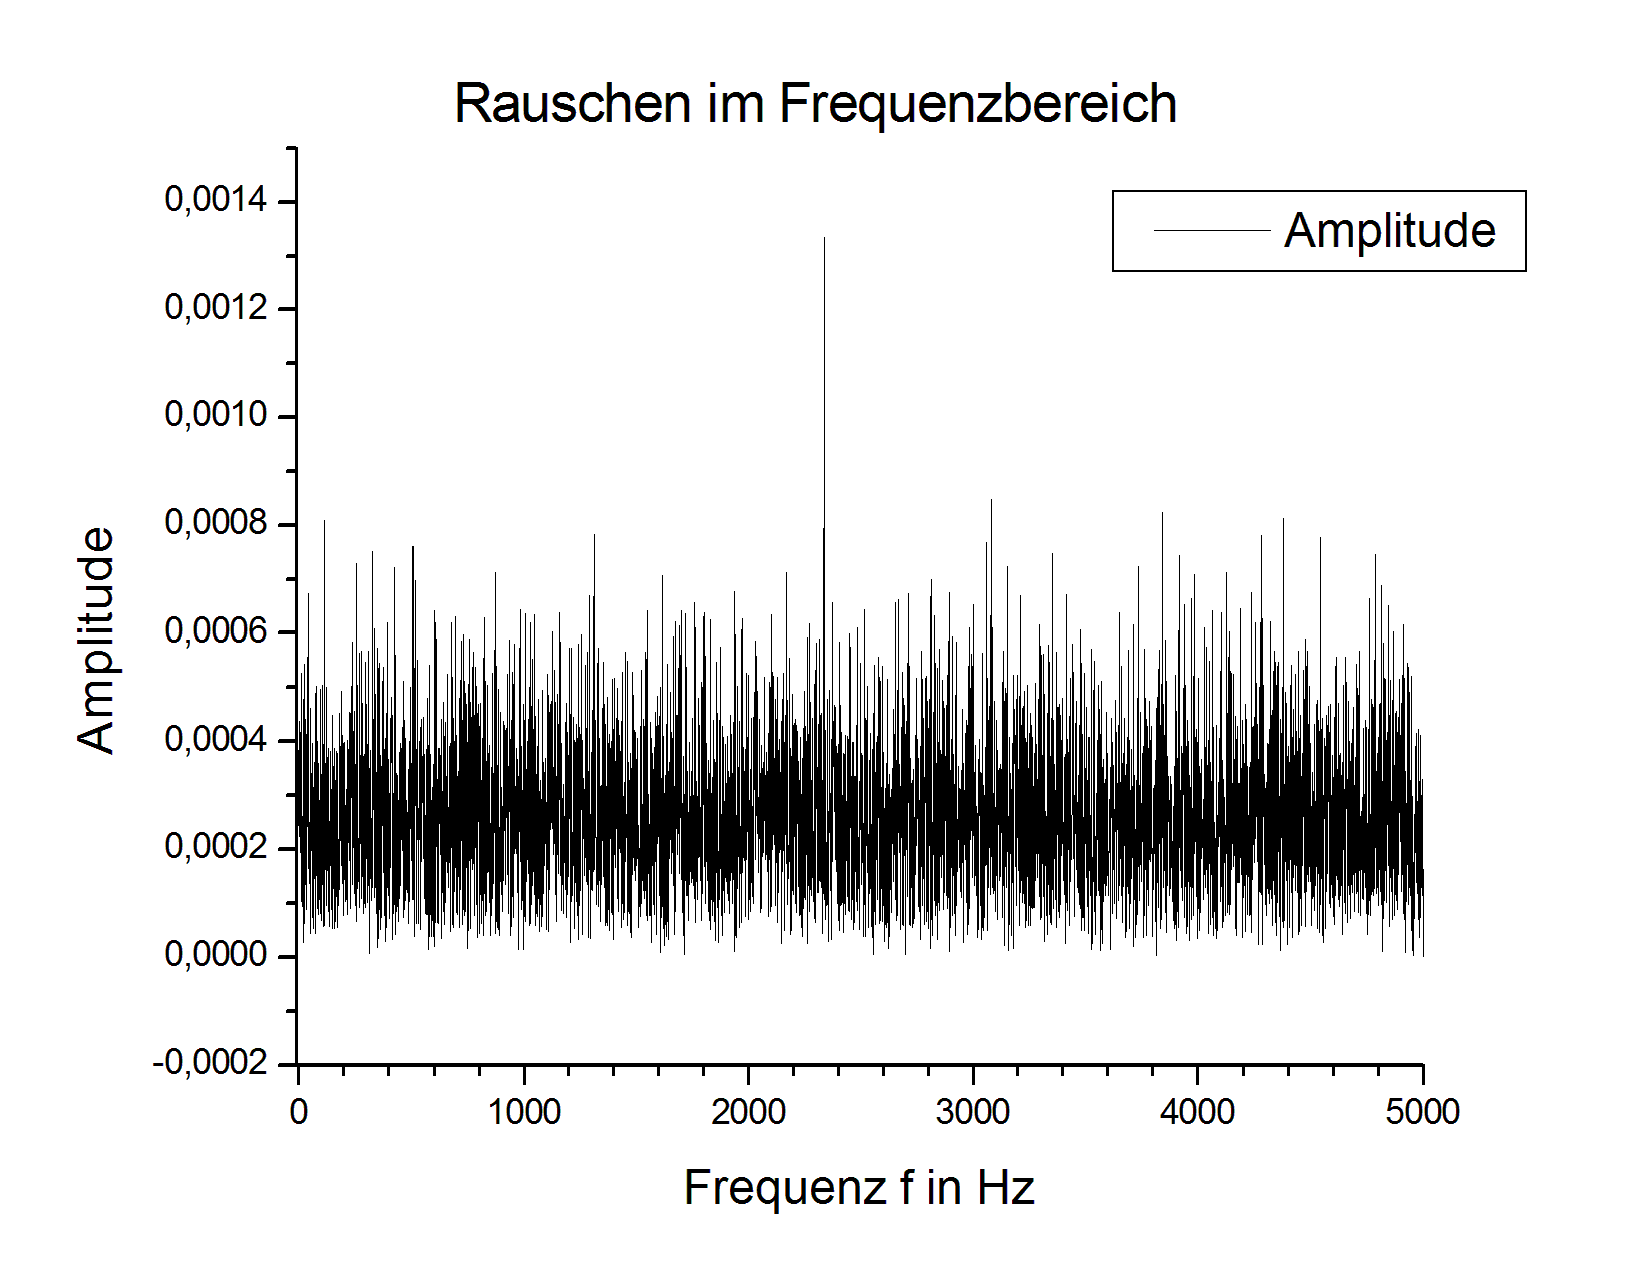
\includegraphics[scale=0.35]{A1c-Graph}
				\caption{Weißes Rauschen im Frequenzbereich}
			\end{figure}
			
			
			\subsubsection{Aufgabe 1.2 - Lock-in zur Detektion kleiner Signale}
			In der nächsten Aufgabe sollte der Lock-in in seiner Anwendung zur Detektion kleiner Signale genutzt werden. Als Modulationseinrichtung wurde ein LED Modulator verwendet, der mit einem langsam veränderlichen Signal (1Hz, sinus, 5$ V $) gespeist wurde. Dies lies die Helligkeit der LED langsam, aber merklich anschwellen und abschwellen. Mithilfe einer Photodiode, welche mit einem $ R=1 \ M\Omega $-Widerstand parallel geschaltet wurde, konnte das Signal gelesen, und am Oszilloskop dargestellt werden. In diesem Aufbau konnte man das Signal nur erkennen, wenn man die Photodiode unmittelbar vor/an die LED gehalten hat:\\
			\begin{figure}[h!b!]
				\centering
				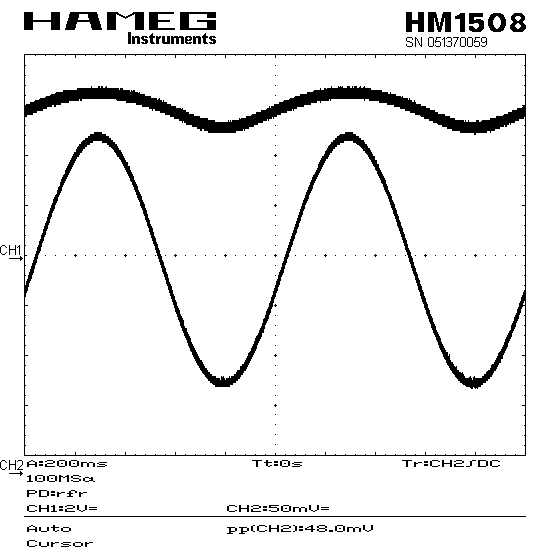
\includegraphics[scale=0.40]{Signal-unmoduliert}
				\caption{unmoduliertes Signal mit $U=5\, V $, unmittelbar vor LED}
			\end{figure}
			Hierbei ist das größere Signal das Eingangssignal (1Hz), und das nach oben verschobene Signal das Photodiodensignal. Es zeigt sich,dass die Amplitude des an der Photodiode aufgezeichneten Signals mit $ U_2= 48\,mV_{pp}$ wesentlich geringer ist, als das abgestrahlte Signal mit einer Spannungsamplitude von $ U_1=10 \, V_{pp} $. Daher haben wir uns im späteren Versuchsteil entschlossen eine Spannung von $U=10\,V$ anzulegen, um das Signal unmittelbar vor dem LED-Modulator deutlicher zu erkennen.\\
			Nun wurde zusätzlich eine Modulationsfrequenz von $ f_{mod}=10\,Hz$ angelegt.  Was diese mit dem Signal macht, ist in nachfolgenden Bildern veranschaulicht.
			\begin{figure}[h!]
				\centering
				\subfigure[$f_{mod}=10\,Hz \ , \ U_1=10\,V_{pp} \ , \ Abstand: \ 0\,cm $]{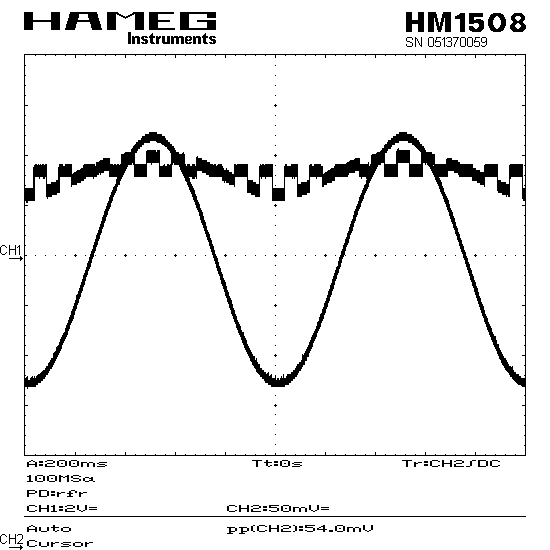
\includegraphics[scale=0.39]{moduliert10Hz-0cm}}
				\subfigure[$ f_{mod}=10\,Hz \ , \ U_1=10\,V_{pp} \ , \ Abstand: \ 10\,cm $]{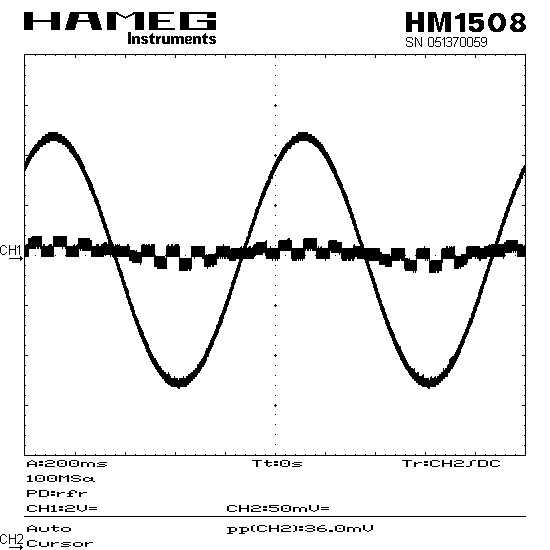
\includegraphics[scale=0.39]{moduliert10Hz-10cm}}
			\end{figure}
			Da die Modulationsfrequenz so gering gewählt ist, kann man deutlich erkennen, wie das Signal " zerhäckselt "/gepulst wird. Die Photodiodenspannung ist dabei von $ U_{2,0cm}=54,0 \,mV_{pp} $ auf $ U_{2,10cm}=36,0 \,mV_{pp} $  gesunken.
			Nun haben wir die Eingangsamplitude erhöht auf $ U_1=10V $ und fanden für diesselben Einstellungen wie oben:\\
			\begin{figure}[h!b!]
				\centering
				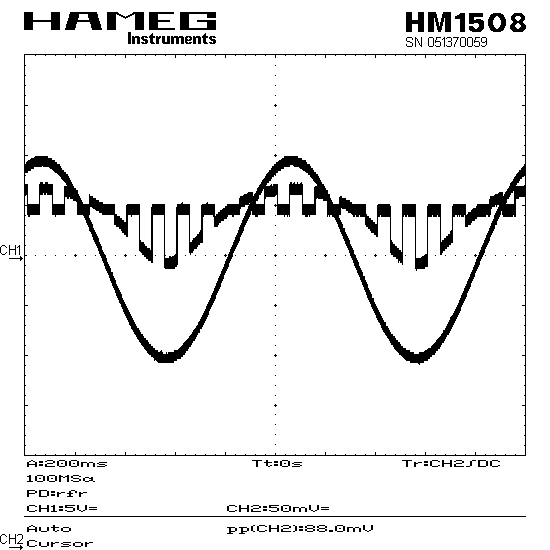
\includegraphics[scale=0.4]{moduliert10Hz-10Vpp-0cm}
				\caption{$f_{mod}=10\,Hz \ , \ U_1=20\,V_{pp} \ , \ Abstand: \ 0\,cm $}
			\end{figure}
			Die Photodiodenspannungsamplitude ist mit $ U_2=88,0\,mV{pp} $ noch immer klein gegenüber der Eingangsspannung, jedoch deutlich besser zu erkennen als zuvor.\newline
			In Aufgabe 1.2.b haben wir nun den maximal möglichen Abstand bestimmt, für den das unmodulierte Signal noch auflösbar ist. Im Prinzip ist die Lösung schon in Abbildung b) der letzten Seite dargestellt. Denn zunächst haben wir rein optisch geurteilt, bis wann noch eine Schwingung erkennbar ist. Dies war bei einem Abstand von 10cm der Fall.\newline
			Für Aufgabe 1.2.c haben wir uns schließlich entschieden, dass wir die Entfernung l messen, bei der die Amplitude der Photodiode auf 10\% der Amplitude direkt vor der LED (l=0) abgefallen ist. Im Nachhinein war diese Entscheidung nicht besonders günstig. Die Eingangsspannung des LED Modulators blieb bei $ U_1=10\,V_{pp} $. Für eine Modulationsfrequenz von 180\,Hz, war mit dem Breitbandverstärker die Amplitude $ U_2(l=0\,cm)\approx128\,mV $ in l=25\,cm auf $ U_2(l=25\,cm)\approx12,8\,mV $ abgefallen [kein Bild aufgenommen]. Nur wenige Zentimeter weiter entfernt, war das Signal nicht mehr auflösbar. Für den exakteren Schmalbandverstärker mit dem hinzugeschalteten TT-Filter für 180Hz war hingegen - und das lässt an dem Bewertungskriterium zweifeln - schon in l=17\,cm die Spannungsamplitude der Photodiode von $ U_2(l=0\,cm)\approx24,3\,V $ [!!!] auf $ U_2(l=17\,cm)\approx2,4\,V $ gefallen. Dies ist in nachfolgenden Diagrammen illustriert.\\
			\begin{figure}[h!]
			\centering
				\subfigure[Schmalbandverstärker, l=0cm]{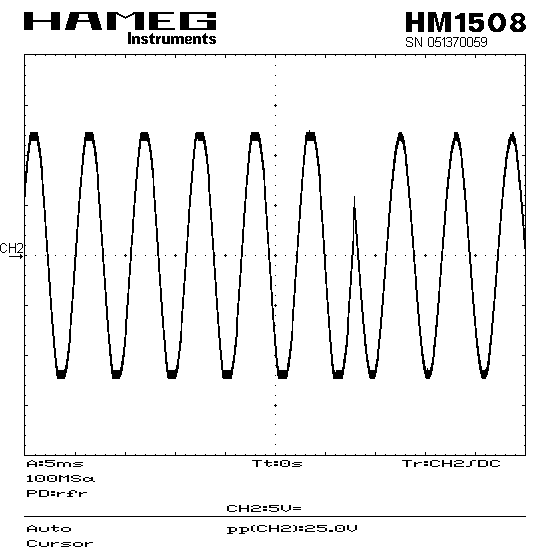
\includegraphics[scale=0.4]{fmod=180Hz-Schmalband-0cm}}
				\subfigure[Schmalbandverstärker, l=17cm]{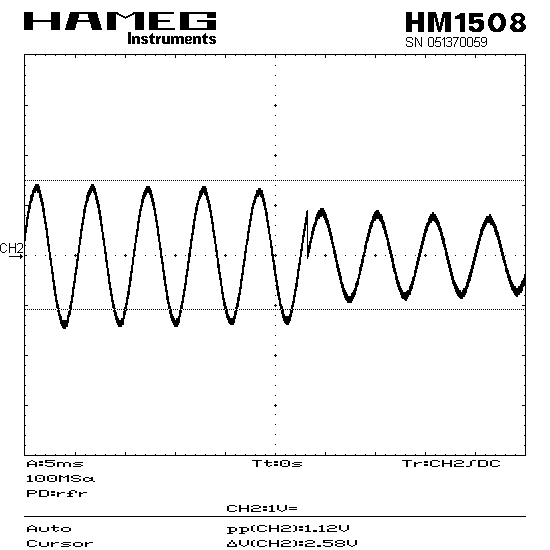
\includegraphics[scale=0.4]{fmod=180Hz-Schmalband-17cm}}
			\end{figure}
			Es lassen sich in beiden Diagrammen Unstetigkeiten erkennen. Diese Entstehen jedoch dadurch, dass LED Modulator und Photodiode nicht fest justiert sind, sondern von den Experimentatoren per Hand gehalten und ausgelenkt werden (->Diskussion).
			Jedoch am Ende des Tisches in 1\,m Entfernung ergab sich noch folgendes, unten dargestelltes, auflösbares Signal. Rechts daneben ist im Vergleich das "Nullpunktsrauschen" der Photodiode aufgenommen, d.h. das Ausgangssignal bei ausgeschaltetem LED-Modulator. Wie man gut erkennt, ist das Signal durchaus noch auflösbar und unterscheidet sich sowohl in Intensität, als auch in der Form von dem Nullpunktsrauschen.\clearpage
			\begin{figure}[h!t!]
					\centering
					\subfigure[Schmalbandverstärker, l=1\,m]{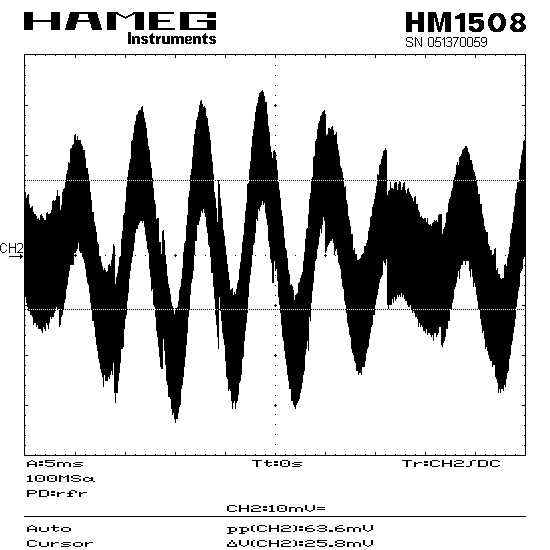
\includegraphics[scale=0.4]{fmod=180Hz-Schmalband-1m}}
					\subfigure[Schmalbandverstärker, Nullpunktsrauschen]{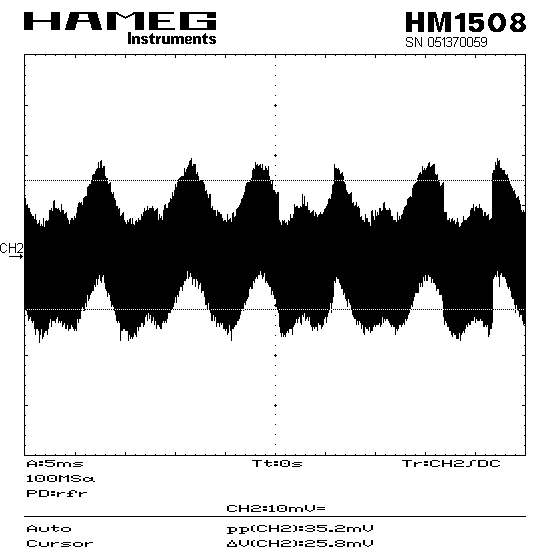
\includegraphics[scale=0.4]{Nullpunktsrauschen-Schmalband}}
			\end{figure}
			Zum Schluss verwendeten wir in Aufgabenteil 1.2.d) den vollständigen Lock-in, mit dem TT-Filter 180Hz. Da direkt vor der LED die Ausgangsspannung ungeheuer groß wurde, haben wir außnahmsweise bei l=2\,cm mit $ U_2(l=2cm)=15,7\,V $ unseren "Nullpunkt" gesetzt. Jedoch schon nach l=19\,cm ist die Spannung auf 10\% des Ausgangswertes abgefallen. \\
			Dann testeten wir, in welcher Entfernung das Signal noch auflösbar war. Dazu nahmen wir die Kabelrolle mit dem BNC-Kabel und versuchten das Signal aufzufangen. Dies war durch den gesamten Versuchsraum möglich und noch gut auflösbar. Also kann man qualitativ für die maximal auflösbare Distanz nur sagen: $ >7,5\,m $. Ein interessanter Test wäre es gewesen, wenn wir für fest-justierte und ausgerichtete LED-Modulator und Photodiode die maximal mögliche Distanz ausgetestet hätten (Gang, etc.). Denn da Potential des Lock-in ist wesentlich größer.\newline
			\\
			Die dritte Aufgabe 1.3 sollte nicht bearbeitet werden.
			
	\clearpage

\section{Diskussion}
- ZUsammenhang Standardabweichung Rauschen vor Lock-in und nach Lock-in überlegen (Aufgabe 1.1.c) \\
				- z.B. Verluste des LED-Modulators...\\
				- schlechte Wahl des Bewertungskriteriums -- besser SNR=1\\
				- Unstetigkeiten in den Diagrammen ... wackler und halten des LED-Modulators und der Photodiode mit der Hand\\
				- Woher kommen die Schwingungen im "Nullpunktssignal" des Schmalbandverstärkers??? - andere Versuchsplätze oder so...
				
\end{document}